%----------------------------------------------------------------------------------------
%	PACKAGES AND THEMES
%----------------------------------------------------------------------------------------
\documentclass[aspectratio=169,xcolor=dvipsnames, t, spanish]{beamer}
\usepackage{fontspec} % Allows using custom font. MUST be before loading the theme!

\usetheme{SimplePlusAIC}
\usepackage{hyperref}
\usepackage{graphicx} % Allows including images
\usepackage{booktabs} % Allows the use of \toprule, \midrule and  \bottomrule in tables
\usepackage{svg} %allows using svg figures
\usepackage{tikz}
\usepackage{makecell}
\usepackage{wrapfig}

\newcommand{\indep}{\perp \!\!\! \perp}
\newcommand{\X}{\mathcal{X}}
\newcommand{\HH}{\mathcal{H}}
\newcommand{\B}{\mathcal{B}}
\newcommand{\C}{\mathbb{C}}
\newcommand{\R}{\mathbb{R}}
\newcommand{\Q}{\mathbb{Q}}
\newcommand{\Z}{\mathbb{Z}}
\newcommand{\N}{\mathbb{N}}
\newcommand{\E}{\mathbb{E}}
\newcommand{\PP}{\mathbb{P}}

% ADD YOUR PACKAGES BELOW
\usepackage{dsfont}
\usepackage[authoryear]{natbib} % Added for proper citations


%----------------------------------------------------------------------------------------
%	TITLE PAGE CONFIGURATION
%----------------------------------------------------------------------------------------

\title[short title]{Modelos Generativos} % The short title appears at the bottom of every slide, the full title is only on the title page
\subtitle{MA5606: Tópicos Matemáticos en Aprendizaje de Máquinas, Redes Neuronales y Aprendizaje Profundo}

\author[Surname]{Joaquín Fontbona, Claudio Muñoz, Diego Olguín, Álvaro Márquez y Javier Maass}
\institute[DIM Universidad de Chile]{Departamento de Ingeniería Matemática \newline Universidad de Chile}
% Your institution as it will appear on the bottom of every slide, maybe shorthand to save space


\date{12 de junio} % Date, can be changed to a custom date
%----------------------------------------------------------------------------------------
%	PRESENTATION SLIDES
%----------------------------------------------------------------------------------------
\usepackage[spanish]{babel}
%\usepackage[T1]{fontenc}
\begin{document}

\maketitlepage

\begin{frame}[t]{Contenidos}
    \tableofcontents
\end{frame}


%------------------------------------------------
\makesection{Modelos Generativos}

\begin{frame}{Generemos motivación}
\begin{center}
    Digamos que tenemos datos que vienen dados por una distribución $\pi$ (e.g. fotos de perros y gatos, todos los textos de literatura latinoamericana existentes, todas las películas de StarWars, una gaussiana, etc.).
    \vspace{2mm}

    \begin{minipage}{0.48\textwidth}
    \begin{center}
        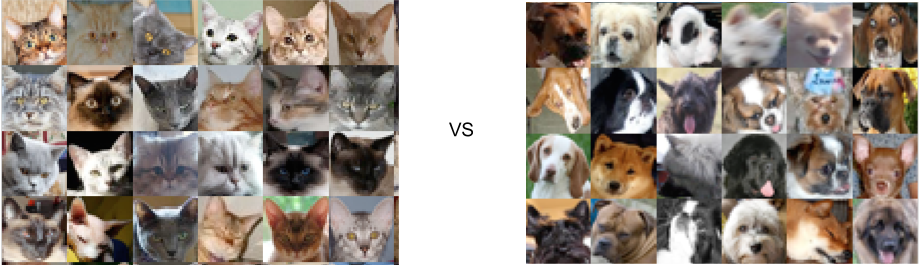
\includegraphics[width=\textwidth]{figures/CatsDogs.png}
    \end{center}
    \end{minipage}\begin{minipage}{0.45\textwidth}
    \begin{center}
        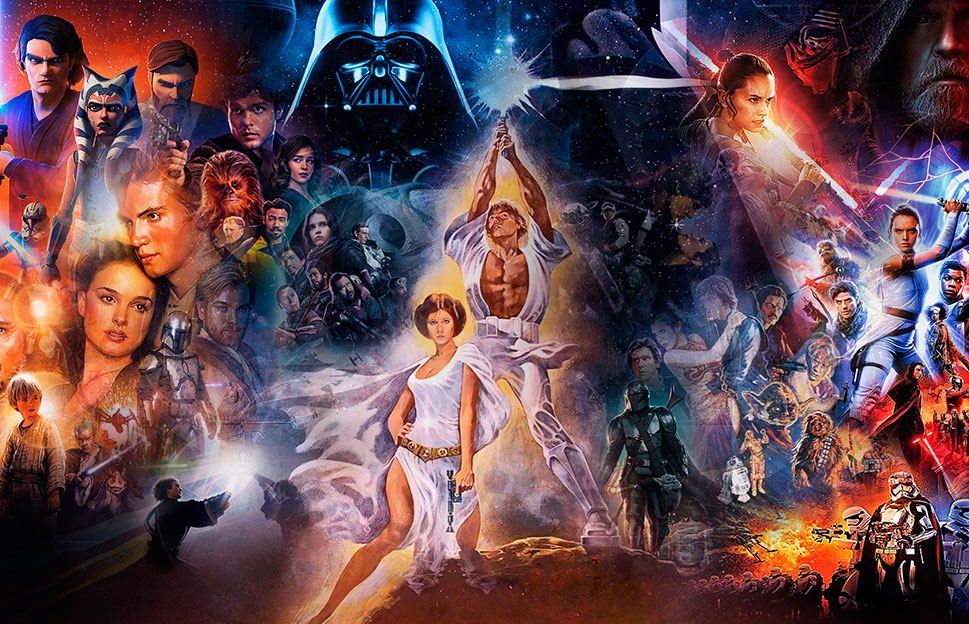
\includegraphics[width=0.6\textwidth]{figures/Star-Wars-Day-2-web.jpg}
    \end{center}
    \end{minipage}\vspace{2mm}

    \pause

    ¿Y si quisiéramos \textbf{generar un nuevo dato de forma natural}? i.e. ¿si quisiéramos \textit{samplear} de nuestra distribución $\pi$?
    
    \pause
    
    Aparecen los \textbf{Modelos Generativos} al rescate!
\end{center}
\end{frame}

\begin{frame}{Generemos motivación}
\begin{center}
    Pero, \textbf{¿por qué querríamos \textit{samplear} datos desde $\pi$?}
\end{center}
\begin{itemize}
        \item La tecnología nos ayuda a automatizar tareas que nunca imaginamos! ¿Y si quisiéramos automatizar el \textit{arte}?
        \pause

        \item ¿Y si quisiéramos generar fotos de perros?\vspace{2mm}\pause
        \begin{center}
            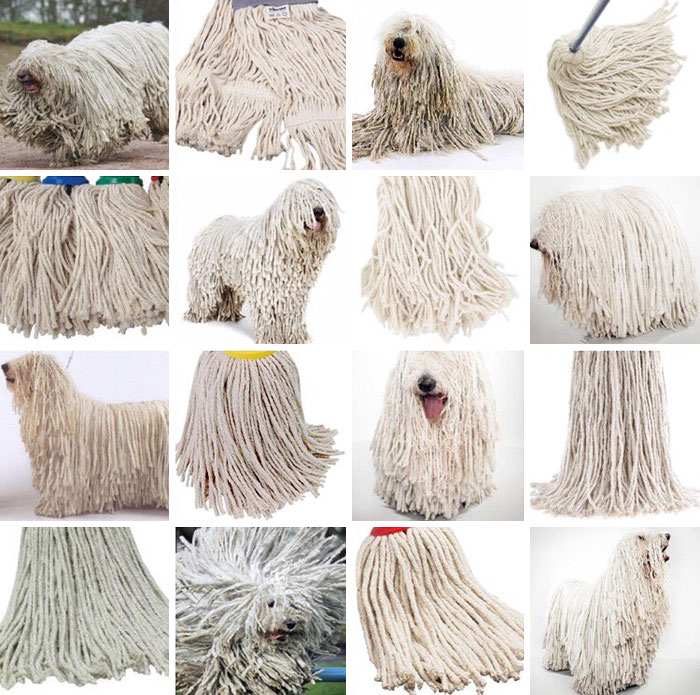
\includegraphics[width=0.5\textwidth,trim={0cm 12.5cm 0cm 0cm},clip]{figures/PerrosMopas.jpg}
        \end{center}
    \end{itemize}
\end{frame}

% \begin{frame}{Generemos motivación}
% \begin{center}
%     ¿Y si quisiéramos lograr la paz en el mundo?
%     \pause
% \end{center}
%     \begin{minipage}{0.5\textwidth}
%         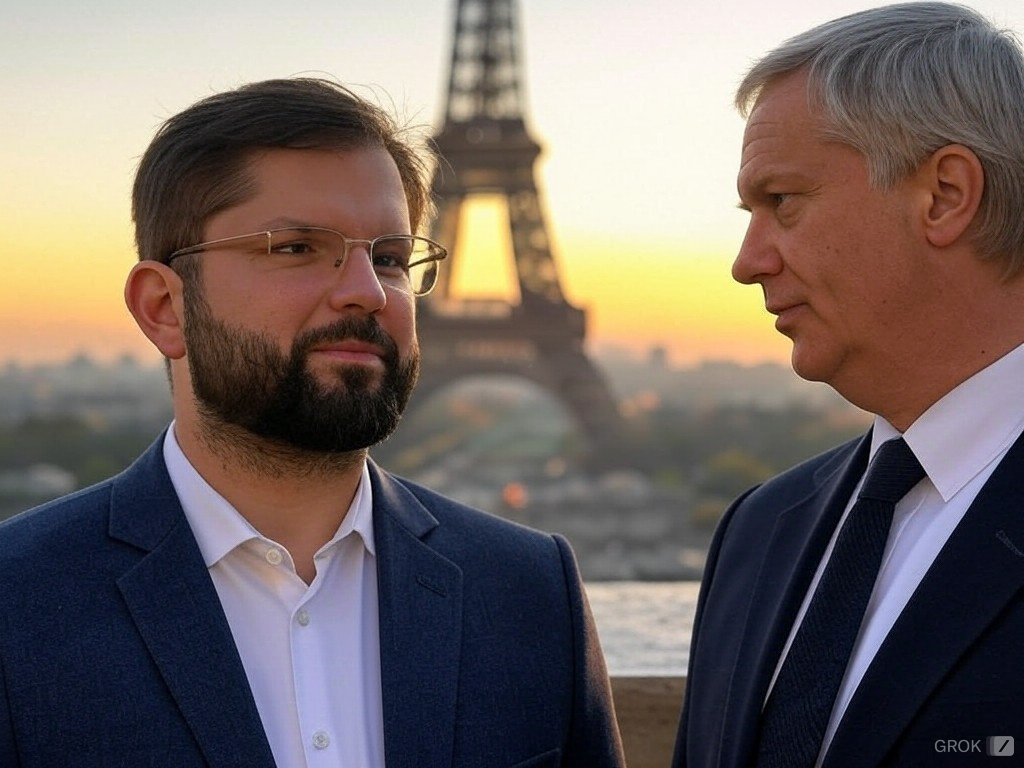
\includegraphics[width=0.9\textwidth]{figures/BoricKast.jpeg}
%         \pause
%     \end{minipage}\begin{minipage}{0.5\textwidth}
%         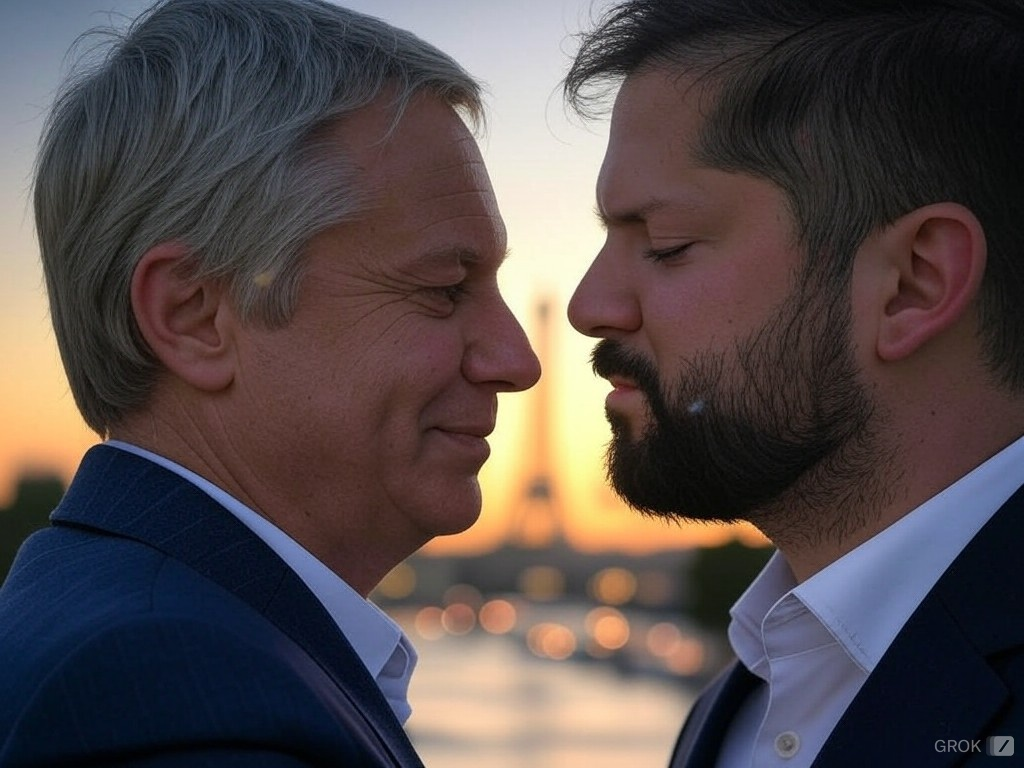
\includegraphics[width=0.9\textwidth]{figures/BoricKastBeso.jpeg}
%     \end{minipage}
% \end{frame}

\begin{frame}{Generemos motivación}
\begin{center}
    ¿Y si pudiésemos hacer los sueños realidad?
    \pause
\end{center}
    \begin{figure}
        \centering
        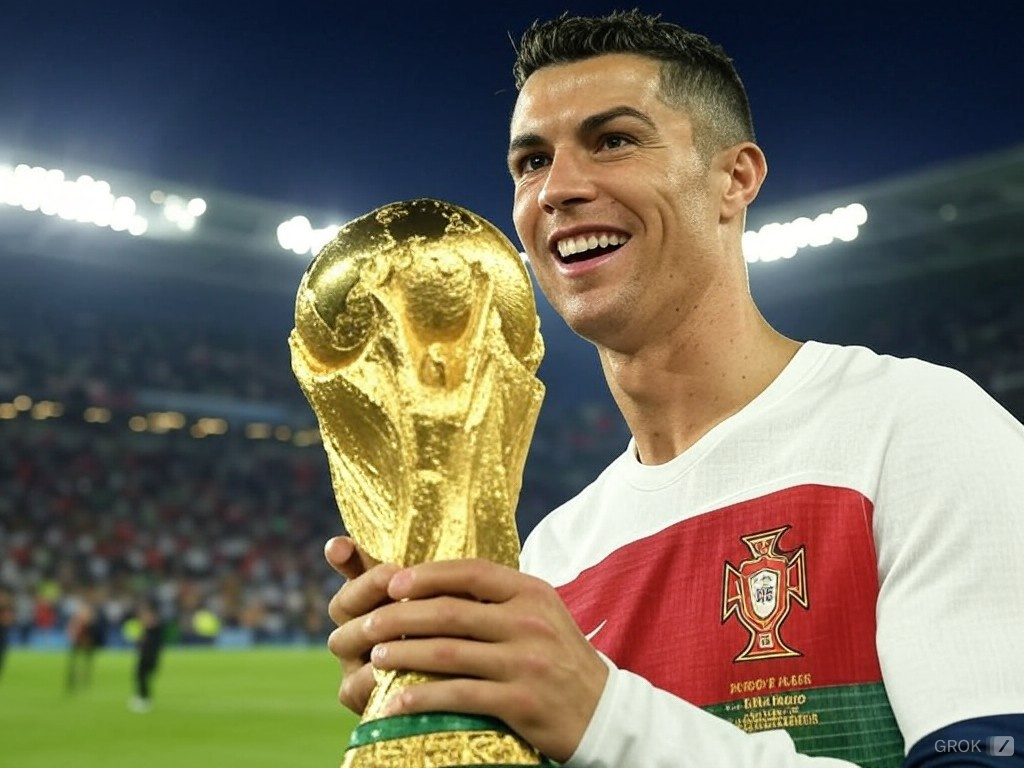
\includegraphics[width=0.5\linewidth]{figures/CristanoCopaDelMundo.jpeg}
    \end{figure}
\end{frame}

\begin{frame}{Generemos motivación}
\begin{center}
    Más allá de los ejemplos ````graciosos'''', la idea principal de los \textbf{Modelos Generativos} es intentar tener modelos que \textbf{entiendan muy bien una distribución de datos}, al punto que nos permitan incluso \textbf{samplear desde ella}.
    \vspace{2mm}
    
    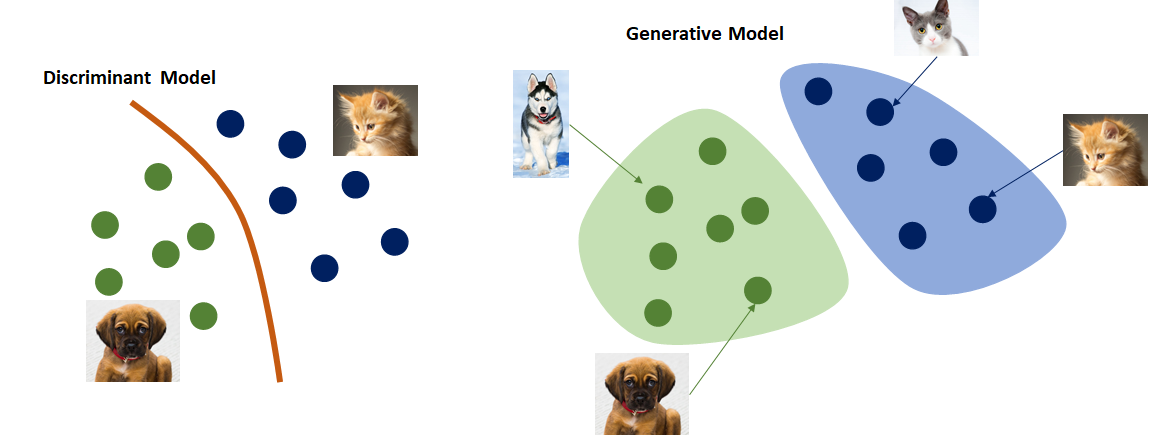
\includegraphics[width=0.8\textwidth]{figures/GenvsDisc.png}
\end{center}
\end{frame}

\begin{frame}{Generemos motivación}\vspace{-6mm}
\begin{center}
    Existen \textbf{varios tipos de Modelos Generativos}:
    \vspace{2mm}
    
    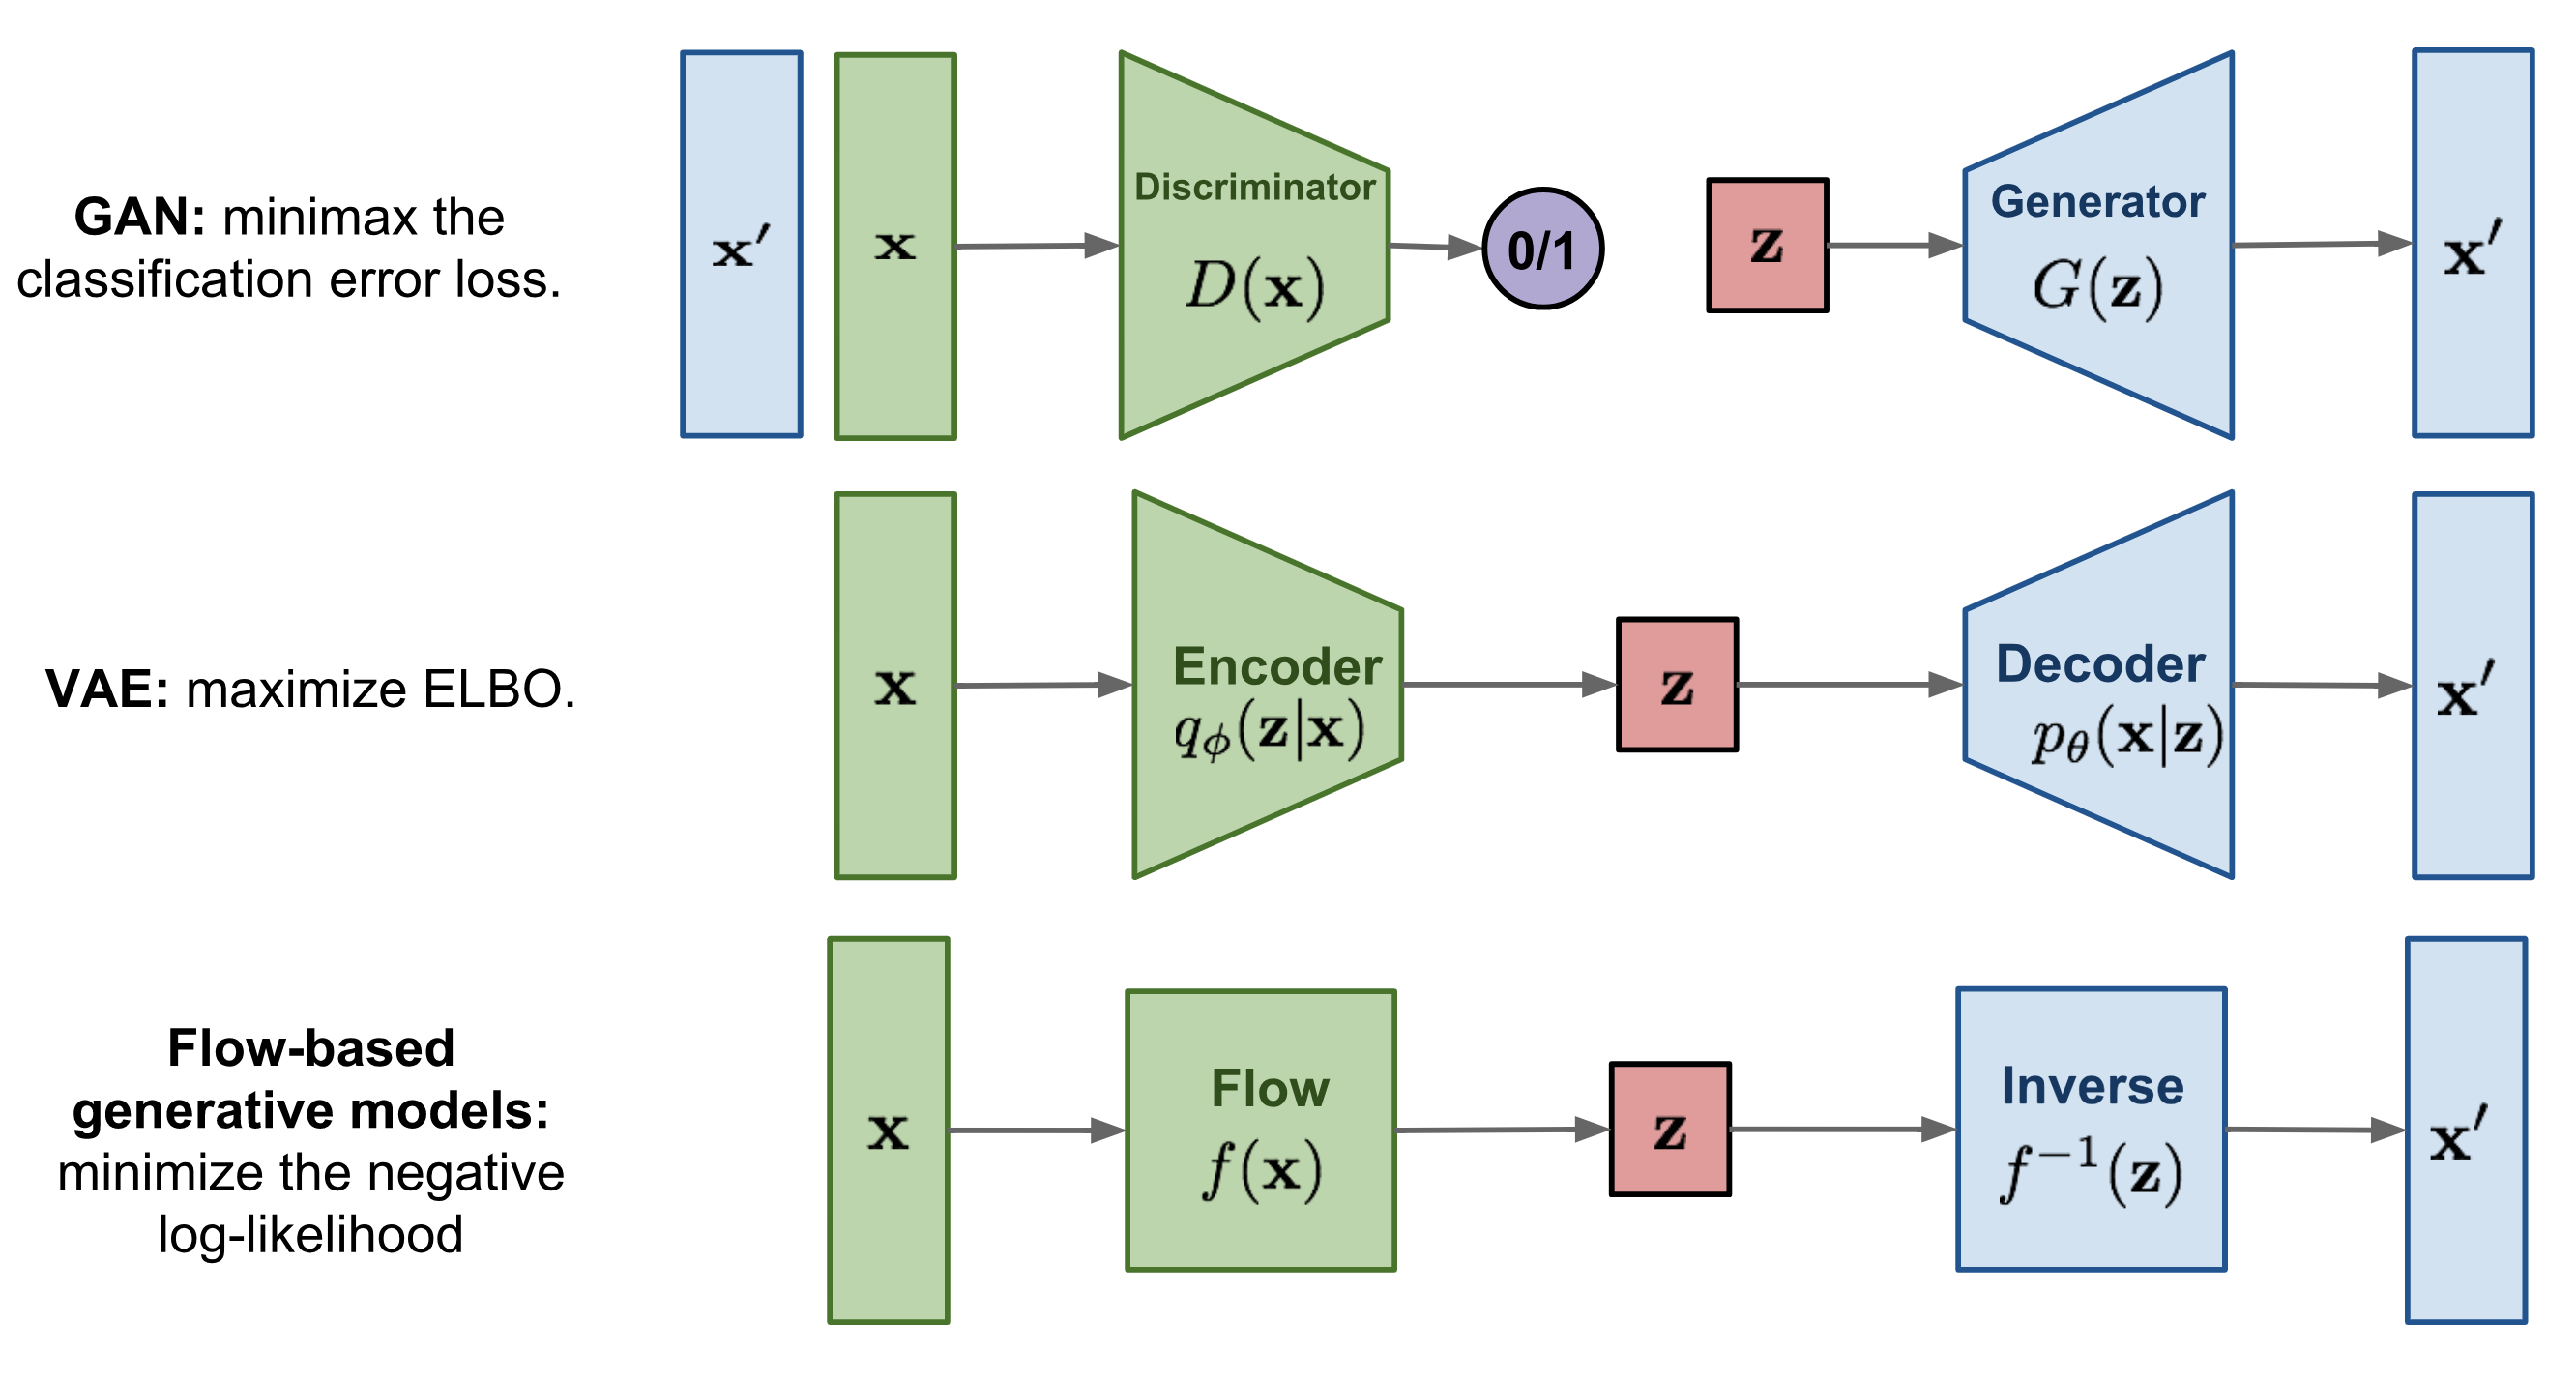
\includegraphics[width=0.6\textwidth]{figures/GenModels.png}
    \vspace{2mm}

    En este tutorial exploraremos principalmente las \textbf{GANs} y los \textbf{Modelos de Difusión}.
\end{center}
\end{frame}

%------------------------------------------------
\makesection{Generative Adversarial Networks (GANs)}

\begin{frame}{Redes Generativas Adversarias (GANs)}
    \begin{center}
        Las slides de esta sección están fuertemente basadas en la sección de GANs del trabajo de tesis de Francisco Muñoz (\cite{MunozLopez2024}).

        Si bien me tocó adaptar el material, los créditos de la autoría y las fuentes recabadas son para él.
    \end{center}
\end{frame}

% Introducción
\begin{frame}{Introducción a GANs}
    \begin{itemize}
        \item Las Redes Generativas Adversarias (\textbf{GANs}), proponen un marco de entrenamiento donde dos redes neuronales compiten entre sí.
        \pause
        \item Se basan en un juego min-max entre dos redes:
        \pause
        \begin{itemize}
            \item \textbf{Generador (G)}: Aprende a generar datos similares a los reales.
            \pause
            \item \textbf{Discriminador (D)}: Aprende a distinguir entre datos reales y generados.
        \end{itemize}
        \pause
        \item Esta arquitectura fue propuesta inicialmente por \citet{Goodfellow2014}; y ha sido objeto de estudio extensivo desde entonces (\citet{Arjovsky2017}; \citet{Gulrajani2017}; \citet{Heusel2017}; \citet{Salimans2016}; \citet{Zhu2017}; \citet{Wang2018}; \citet{Xiao2021}; entre muchos otros).
    \end{itemize}
\end{frame}

\begin{frame}{Esquema de las GANs}
    \begin{figure}
        \centering
        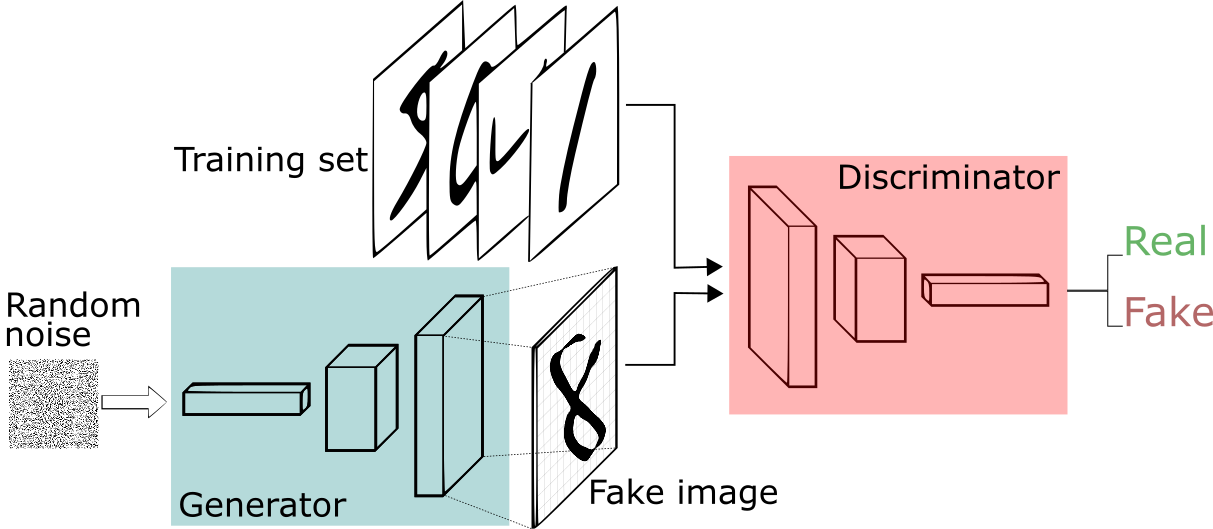
\includegraphics[width=0.9\linewidth]{figures/GANs.png}
        \label{fig:enter-label}
    \end{figure}
\end{frame}


\begin{frame}{Definición Formal de una GAN}\vspace{-3mm}
    \begin{center}
        Plantearemos la idea de las GANs en un contexto \textbf{no paramétrico}, basado en medidas de probabilidad generales, sin ahondar todavía en las NNs como tal.
    \end{center}
    \pause
    \begin{block}{Planteamiento de Teoría de Juegos}
    Dado $(\mathcal{X}, \pi)$ e.d.p., una GAN es un juego de \textbf{suma cero} con dos jugadores:
            \begin{itemize}
                \item Un \textbf{G}enerador $\mu_{G}$, con un conjunto de estrategias $\mathcal{P}(\mathcal{X})$.
                \item Un \textbf{D}iscriminador $\mu_{D}(\cdot|x)$, con kernels Markovianos a $[0,1]$ como estrategias.
            \end{itemize}
    La función valor objetivo del juego es:   
    $$V(\mu_{G},\mu_{D})=\mathbb{E}_{X\sim\pi}\mathbb{E}_{Y\sim\mu_{D}(X)}[\ln~Y]+\mathbb{E}_{\tilde{X}\sim\mu_{G}}\mathbb{E}_{Y\sim\mu_{D}(\tilde{X})}[\ln(1-Y)]$$ 
    La cual es \textbf{minimizada por G} y \textbf{maximizada por D}. 
    \end{block}
\end{frame}

\begin{frame}{Definición Formal de una GAN}

\begin{theorem}[Discriminador Óptimo]
Para un generador fijo $\mu_G$, el discriminador óptimo (que \textbf{existe y es único}) es:
\[
\mu_D^*(\cdot|x) = \delta_{D^*(x)}(\cdot),\;\; \text{ donde } \;\; D^*(x) = \frac{d\pi}{d(\mu_G + \pi)}(x)
\]
Es decir, es una función determinista $D^*:\mathcal{X} \to [0,1]$. En este caso, se tiene:
\[
V(\mu_G, \mu_D^*) = \text{JS}(\pi, \mu_G) - 2\ln 2
\]
con $\text{JS}$ la \textbf{divergencia de Jensen-Shannon} entre 2 medidas.
\end{theorem}
\pause
\begin{center}
    Es decir, \textbf{el discriminador busca distinguir muestras verdaderas de falsas de la mejor forma posible}.
\end{center}
\end{frame}

\begin{frame}{Definición Formal de una GAN}\vspace{-2mm}
\begin{block}{Esquema de demostración del Teorema del Discriminador Óptimo}
Usando desigualdad de Jensen y lema de Doob:
\begin{enumerate}
\item Maximizar $V(\mu_G, \mu_D)$ sobre $\mu_D$ equivale a maximizar (\textbf{s.p.g}): \vspace{-1mm}
\[
\max_{D: \mathcal{X}\to[0,1]} \mathbb{E}_{X\sim \pi}[\ln D(X)] + \mathbb{E}_{\tilde{X}\sim \mu_G}[\ln(1-D(\tilde{X}))]
\]
\item Como la función $y\mapsto a\ln y+b\ln(1-y)$ alcanza su máximo en $y^{*}=\frac{a}{a+b}$; la solución óptima se obtiene cuando: \vspace{-2mm}
        $$D^{*}(x)=\frac{d\pi}{d(\pi+\mu_{G})} (x)$$

\item Sustituyendo en $V$ se obtiene la relación con $JS(\pi, \mu_G)$
\end{enumerate}
\end{block}
\end{frame}


\begin{frame}{Definición Formal de una GAN}\vspace{-7mm}
\begin{center}
    Dado el teorema, podemos definir: $C(\mu_G) := V(\mu_G, \mu_{D}^*) = \text{JS}(\mu, \mu_G) - 2 \ln 2$
\end{center}
\pause
\begin{theorem}[Generador Óptimo]
El mínimo global de la función $C(\mu_{G})$ se alcanza en $\mu_{G}^{*}=\pi$, y el valor del mínimo es $C(\pi)=-\ln4$. i.e. \textbf{El mejor generador posible es uno que imita perfectamente $\pi$}.
\end{theorem}
\pause
\begin{block}{Demostración}
    \begin{itemize}
        \item Partiendo del Teorema anterior: \vspace{-2mm}
        $$\min_{\mu_{G}}\max_{\mu_{D}}V(\mu_{G},\mu_{D}) = \min_{\mu_{G}}V(\mu_{G},\mu_{D}^{*}) = \min_{\mu_{G}}C(\mu_{G})= \min_{\mu_{G}}JS(\pi,\mu_{G})-2\ln2 \vspace{-2mm}$$ 
        \item Como la divergencia de Jensen-Shannon es estrictamente positiva si $\mu_{G}\ne\pi$, y nula si $\mu_{G}=\pi$, entonces el mínimo global de $C(\mu_{G})$ se alcanza en $\mu_{G}^{*}=\pi$. 
        \item El valor mínimo es $C(\pi)=-\ln4$. 
    \end{itemize}
\end{block}
\end{frame}

% Definición de Redes
\begin{frame}{Implementación Práctica de las GANs}
\begin{block}{Planteamiento Funcional del Problema}
    \begin{itemize}
        \item \textbf{El discriminador se puede buscar como una función $D:\mathcal{X}\to[0,1]$}. 
        \item Análogamente, en la práctica el \textbf{generador óptimo se plantea como una pushforward de una distribución conocida}: $\mu_G = G \# \mu_Z$, con $\mathcal{Z}$ un \textit{espacio latente}, $\mu_Z$ una distribución conocida (e.g. \textit{Gaussiana}), y $G:\mathcal{Z} \to \mathcal{X}$ medible. %que \textbf{mapea el ruido desde $\mathcal{Z}$ a $\mathcal{X}$}
    \end{itemize}
\end{block}
\pause
\begin{center}
    En la práctica, aproximamos esto con dos redes neuronales: una con pesos $\theta_g$ que llamaremos \textbf{Generador} y otra con pesos $\theta_d$ que llamaremos \textbf{Discriminador}.
\end{center}
    \pause
    \begin{itemize}
        \item \textbf{Generador (G)}: Define una función $G(z; \theta_g)$ que mapea ruido $z \sim \mu_Z$ a $\mathcal{X}$.
        \pause
        \item \textbf{Discriminador (D)}: Define $D(x; \theta_d)$, que da la probabilidad de que $x$ provenga de $\pi$.
    \end{itemize}
    \begin{center}
    \end{center}
\end{frame}

\begin{frame}{Esquema de las GANs}
    \begin{figure}
        \centering
        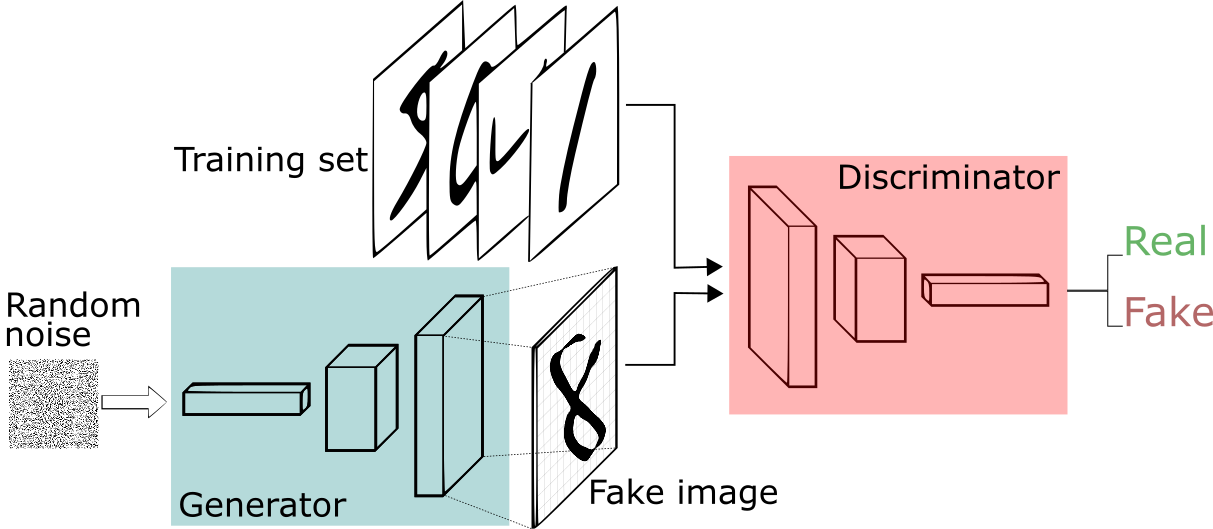
\includegraphics[width=0.9\linewidth]{figures/GANs.png}
        \label{fig:enter-label2}
    \end{figure}
\end{frame}

% Algoritmo General
\begin{frame}{Entrenando a tu GAN}\vspace{-6mm}
\begin{center}
    El entrenamiento de las GANs se realiza usualmente repitiendo $K$ veces el ciclo de: \textbf{Entrenar el Discriminador $\rightarrow$ Entrenar el Generador}, hasta converger.
\end{center}
\pause

    i.e. En cada iteración:
    \begin{itemize}
        \item Muestrear $\{z^{(i)}\}_{i=1}^m$ de la distribución de ruido $\mu_Z$, $\{x^{(i)}\}_{i=1}^m$ de la distribución de datos $\pi$ y actualizar el discriminador según SGD:\vspace{-1mm}
            \[
                \nabla_{\theta_d} \left[ \frac{1}{m} \sum_{i=1}^m \left[ \log D_{\theta_d}\left(x^{(i)}\right) + \log \left(1 - D_{\theta_d}\left(G_{\theta_g}\left(z^{(i)}\right)\right)\right) \right] \right].\vspace{-1mm}
            \]
        \pause
        \item Muestrear $\{z^{(i)}\}_{i=1}^m$ de la distribución de ruido $p_g(z)$ y actualizar según SGD:\vspace{-1mm}
        \[
            \nabla_{\theta_g} \left[\frac{1}{m} \sum_{i=1}^m \log \left(1 - D_{\theta_d}\left(G_{\theta_g}\left(z^{(i)}\right)\right)\right)\right].\vspace{-1mm}
        \]
    \end{itemize}
\end{frame}


\makesection{Denoising Diffusion Models (DDM)}

\begin{frame}{Modelos de Difusión}

    \begin{center}
        Utilizaremos las slides del curso de Generative Modelling de Valentin DeBortoli (\href{https://vdeborto.github.io/project/generative_modeling/}{link})... 

        \pause
        TODAS las slides que vienen a partir de este punto son simplemente una traducción casi verbatim de las slides hechas por Valentin, por lo que no me hago creer el autor de ellas bajo ninguna circunstancia.
    \end{center}
    
\end{frame}

\begin{frame}{Modelos de Difusión}\vspace{-6mm}
    \begin{center}
        \textbf{Denoising Diffusion Models (DDM)} como alternativa para \textbf{generar datos de $\pi$}. También llamados \textbf{Score-Based Generative Models}(ver \href{https://scorebasedgenerativemodeling.github.io/}{aquí} para más referencias).
    \end{center}
        \pause
        
        ¿Por qué elegir este tipo de métodos?:
        \footnotesize
            \begin{itemize}
                \item Resultados \textbf{SOTA} \citet{DhariwalNichol2021}; \citet{Karras2022}.
                \item \textbf{Altamente flexibles} \citet{Poole2022}; \citet{Rombach2022}; \citet{Balaji2022}; \citet{Saharia2022} (aplicaciones en Text2Image, CLIP, entre muchas otras).
                \item \textbf{Garantías Teóricas} \citet{DeBortoli2021b}; \citet{Chen2022}; \citet{Pidstrigach2022}; \citet{Lee2022}.
            \end{itemize}
        ** Eso sí, la \textbf{comprensión estadística} de estos modelos todavía es limitada.
        \pause
    
        \begin{minipage}{0.6\textwidth}
        \begin{figure}
            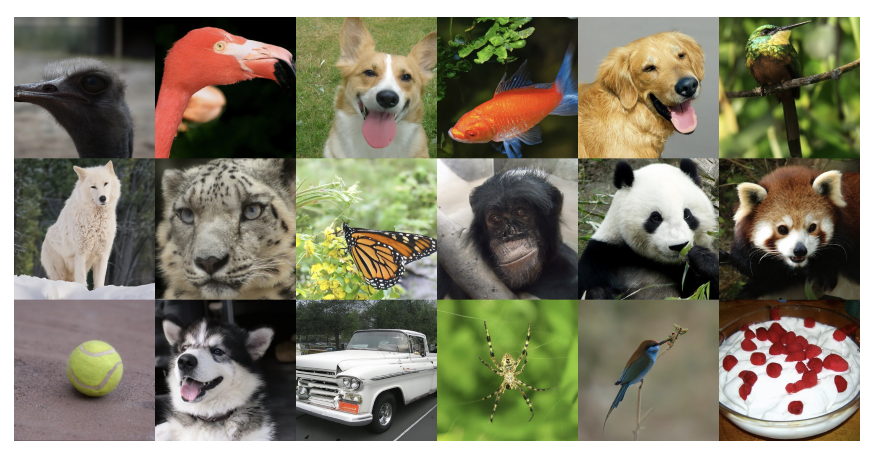
\includegraphics[width=0.5\textwidth]{figures/ImgDiffusion.png}
            \caption{Imagen Generada por DDM \cite{DhariwalNichol2021}.}
        \end{figure}    
        \end{minipage}\begin{minipage}{0.4\textwidth}
        \begin{itemize}
                \item Primer artículo (enfoque variacional) \citet{Sohl-Dickstein2015}.
                \item Primera aplicación exitosa \citet{SongErmon2019}.
                \item Concurrentemente (enfoque variacional) \citet{Ho2020}.
                %\item Nuestra presentación está inspirada en \citet{Song2020b}.  
            \end{itemize}
        \end{minipage}
        
    \end{frame}
    
    % ====================
    % DIAPOSITIVA 7: Principios de DDM
    % ====================
    \begin{frame}{Principios de DDM}\vspace{-6mm}
        \begin{center}
            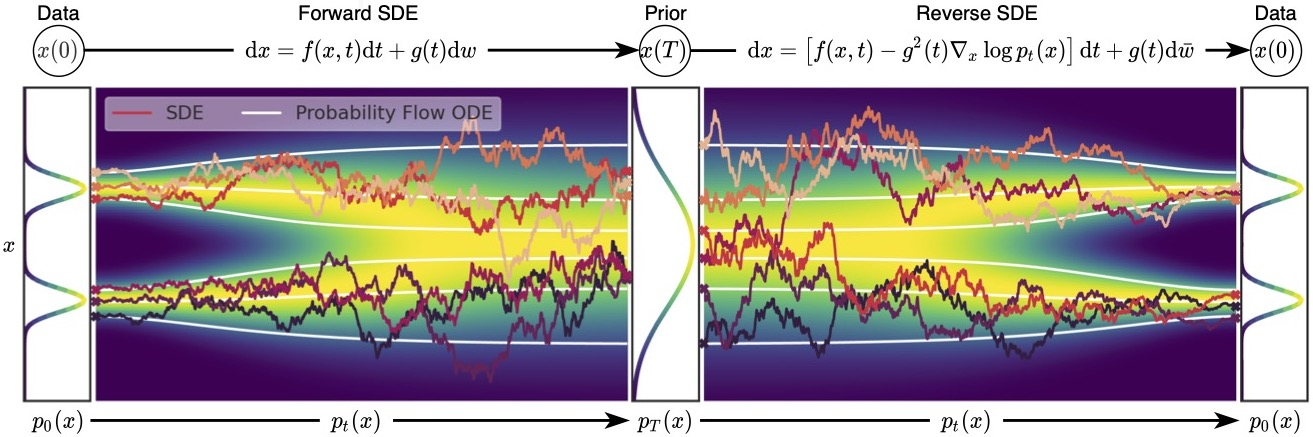
\includegraphics[width=0.7\textwidth]{figures/DDM2.jpg}

            \footnotesize Procesos de ruido y generativos en DDM. Imagen extraída de \citet{Song2020b}.
        \end{center}
        \begin{itemize}
            \item Buscamos \textbf{interpolar} entre dos distribuciones:
            \begin{itemize}
                \item La distribución real de los datos, $\pi\in\mathcal{P}(\mathcal{X})$, y
                \item La distribución \textit{fácil de samplear}, $\mu_Z \in\mathcal{P}(\mathcal{X})$ (e.g. Gaussiana estándar).
            \end{itemize}
            \item Es ``\textbf{fácil}'' ir de $\pi$ a $\mu_Z$, con un \textbf{proceso de \textit{noising} (forward)}.
            \item Queremos \textbf{invertir} este proceso, para ir de $\mu_Z$ a $\pi$, y lograr así un \textbf{proceso generativo}.
        \end{itemize}
    \end{frame}
    
    % ====================
    % DIAPOSITIVA 8: Muestreo ancestral
    % ====================
    \begin{frame}{Ancestral Sampling}\vspace{-6mm}
        \begin{itemize}
            \item Sea $\mathcal{X} = \mathbb{R}^d$, $N\in\mathbb{N}$, $N>0$ y $p$ una densidad en $(\mathbb{R}^{d})^{N+1}$ tal que para cualquier $x_{0:N}=\{x_{k}\}_{k=0}^{N}$, $p$ admite una \textbf{descomposición forward} de la forma:\vspace{-3mm}
            \[ p(x_{0:N})=p_{0}(x_{0})\prod_{k=0}^{N-1}p_{k+1|k}(x_{k+1}|x_{k}) \vspace{-2mm}\]
            \pause\item $\forall k\in\{0,...,N-1\}$ definimos la \textbf{marginal} $p_{k+1}$ para $x_{k+1}\in\mathbb{R}^{d}$\vspace{-1mm}
            \[ p_{k+1}(x_{k+1})=\int_{\mathbb{R}^{d}}p_{k}(x_{k})p_{k+1|k}(x_{k+1}|x_{k})dx_{k} \vspace{-2mm}\]
            \pause\item Asumimos que $\forall k\in\{0,...N\}$, $p_{k}>0$ y definimos $\forall x_{k},x_{k+1}\in\mathbb{R}^{d}$:\vspace{-1mm}
            \[ p_{k|k+1}(x_{k}|x_{k+1})=\frac{p_{k+1|k}(x_{k+1}|x_{k})p_{k}(x_{k})}{p_{k+1}(x_{k+1})}\vspace{-2mm} \]
            \pause\item Podemos obtener la \textbf{descomposición backward}:\vspace{-2mm}
            \[ p(x_{0:N})=p_{N}(x_{N})\prod_{k=0}^{N-1}p_{k|k+1}(x_{k}|x_{k+1}) \]
            %Esto nos permitirá \textbf{samplear trayectorias de $p$ \textit{hacia atrás}}.
        \end{itemize}
    \end{frame}
    
    % ====================
    % DIAPOSITIVA 9: Proceso de ruido
    % ====================
    \begin{frame}{El Proceso Forward}
        \begin{itemize}
            \item En la práctica consideramos:
            \begin{itemize}
                \item $\pi$ admite una densidad $p_{0}$ con respecto a la medida de Lebesgue.
                \item La \textbf{descomposición forward} es un \textbf{proceso de ruido}.\vspace{-2mm}
                \[ p(x_{0:N})=p_{0}(x_{0})\prod_{k=0}^{N-1}p_{k+1|k}(x_{k+1}|x_{k}) \vspace{-2mm}\]
            \end{itemize}
            \pause
            \item ¿Cómo pasamos de la distribución de datos a la distribución fácil de muestrear?
            \begin{itemize}
                \item \textbf{Proceso Autorregresivo}: Para $\{Z_{k}\}_{k\in\mathbb{N}} \sim N(0,Id)$ i.i.d. y $\alpha<1$, hacemos:\vspace{-1mm} \[X_{k+1}=\alpha X_{k}+\sqrt{1-\alpha^{2}}Z_{k+1}\vspace{-1mm}\]
                \item $Law(X_{k})\rightarrow\mathcal{N}(0,Id)$ exponencialmente rápido (en Wasserstein, TV) cuando $k\rightarrow\infty$.
            \end{itemize}
            \pause
            \item Otra forma de verlo:
            \begin{itemize}
                \item Proceso de \textbf{Ornstein-Uhlenbeck}: $dX_{t}=-X_{t}dt+\sqrt{2}dB_{t}$, y su discretización de \textbf{Euler-Maruyama}: $X_{k+1}=(1-\gamma)X_{k}+\sqrt{2\gamma}Z_{k+1}$; la cual converge \textbf{exponencialmente rápido} a $N(0, Id/(1-\gamma/2))$.
            \end{itemize}
        \end{itemize}
    \end{frame}
    
    % ====================
    % DIAPOSITIVA 10: Invirtiendo el proceso de ruido
    % ====================
    \begin{frame}{¿Cómo invertimos el proceso \textbf{forward}?}
    Podemos hacer unos cálculos medios densos, para obtener lo siguiente:
        \begin{align*}
            p_{k|k+1}(x_{k}|x_{k+1}) &= p_{k+1|k}(x_{k+1}|x_{k})p_{k}(x_{k})/p_{k+1}(x_{k+1}) \\
            &= C_{0}\exp[-||x_{k+1}-(1-\gamma)x_{k}||^{2}/(4\gamma)]\exp[\log(p_{k}(x_{k}))-\log(p_{k+1}(x_{k+1}))] \\
            &= C_{1}\exp[-||x_{k+1}-(1-\gamma)x_{k}||^{2}/(4\gamma)]\exp[\log(p_{k}(x_{k}))-\log(p_{k}(x_{k+1}))] \\
            &= C_{1}\exp[-(||x_{k+1}-(1-\gamma)x_{k}||^{2}+4\gamma\{\log(p_{k}(x_{k}))-\log(p_{k}(x_{k+1}))\})/(4\gamma)] .
        \end{align*}\vspace{-3mm}
        
        \pause Donde $C_{0}, C_{1} > 0$ son constantes que dependen solo de $x_{k+1}$. Por otro lado:
        \begin{itemize}
            \item $||x_{k+1}-(1-\gamma)x_{k}||^{2} = ||x_{k}-(1+\gamma)x_{k+1}||^{2}-2\gamma||x_{k+1}-x_{k}||^{2}+\gamma^{2}\{||x_{k}||^{2}-||x_{k+1}||^{2}\}$.
            \item Y, por Taylor: $\log(p_{k}(x_{k}))=\log(p_{k}(x_{k+1}))+\langle\nabla \log p_{k}(x_{k+1}),x_{k}-x_{k+1}\rangle+$ \\ $\int_{0}^{1}\nabla^{2}\log p_{k}((1-t)x_{k+1}+tx_{k})(x_{k}-x_{k+1})^{\otimes2}dt.$
        \end{itemize}
    \end{frame}
    
    % ====================
    % DIAPOSITIVA 11: Invirtiendo el proceso de ruido (2/3)
    % ====================
    \begin{frame}{¿Cómo invertimos el proceso \textbf{forward}?}
        \begin{itemize}
            \item Si \textbf{asumimos} que: $||x_{k+1}-x_{k}||^{2}\le C\gamma$ y $\max(||x_{k}||,||x_{k+1}||)\le C$; entonces:
            \begin{itemize}
                \item $\left| ||x_{k+1}-(1-\gamma)x_{k}||^{2}-||x_{k}-(1+\gamma)x_{k+1}||^{2}\right|\le4C\gamma^{2}.$
                \item $|\log(p_{k}(x_{k}))-\log(p_{k+1}(x_{k+1}))-\langle\nabla \log p_{k}(x_{k+1}),x_{k}-x_{k+1}\rangle|\le D\gamma.$
            \end{itemize}
            \pause
            \item Con eso, \textbf{aproximando} hasta un término de orden $\gamma$ en la exponencial, se tiene:
            \begin{align*}
            p_{k|k+1}(x_{k}|x_{k+1}) &\approx C_{2}\exp\left[-||x_{k}-(1+\gamma)x_{k+1}||^{2}/(4\gamma)+\langle\nabla \log p_{k}(x_{k+1}),x_{k}-x_{k+1}\rangle\right] \\
            &\approx N(x_{k};x_{k+1}+\gamma\{x_{k+1}+2\nabla \log p_{k}(x_{k+1})\},2\gamma Id)
            \end{align*}
            \pause
    
            \item Si bien la aproximación es media rancia, esto nos permite definir de forma simple el \textbf{proceso backward}, desde $X_{N}\sim \mu_Z$:
            \[ X_{k}=X_{k+1}+\gamma\{X_{k+1}+2\nabla \log p_{k}(X_{k+1})\}+\sqrt{2\gamma}Z_{k+1}. \]
            \item Aquí el término $\nabla \log p_{k}$ es \textbf{intractable}, por lo que tendremos que aproximarlo...
        \end{itemize}
    \end{frame}
    
    % ====================
    % DIAPOSITIVA 12: Score-matching (1/4)
    % ====================
    \begin{frame}{Score-matching}\vspace{-3mm}
    \begin{center}
        Al término $\nabla \log p_{k}$ se le conoce como el \textbf{score (de Stein)}; y por eso hablamos de un problema de \textbf{Score-Matching} (ver \citet{Hyvarinen2005}; \citet{Vincent2011}).
    
        Pero, \textbf{¿cómo aprendemos a aproximar algo que es intractable?}
    \end{center}
    \pause
        \begin{itemize}
            \item Usemos la siguiente identidad (ver \citet{Efron2011}):
            \begin{align*}
            \nabla \log p_{k}(x_{k}) &= \nabla p_{k}(x_{k})/p_{k}(x_{k})= \int_{\mathbb{R}^{d}}\nabla \log p_{k|0}(x_{k}|x_{0})p_{0,k}(x_{0},x_{k})dx_{0}/p_{k}(x_{k}) \\
            &= \int_{\mathbb{R}^{d}}\nabla \log p_{k|0}(x_{k}|x_{0})p_{0|k}(x_{0}|x_{k})dx_{0} = \mathbb{E}_{p_{0|k}(\cdot|x_{k})}[\nabla \log p_{k|0}(x_{k}|X_{0})].
            \end{align*}
            \pause
            \item De este modo, tenemos una \textbf{expresión intermedia} más razonable:
            \begin{itemize}
                \item $\nabla \log p_{k|0}(x_{k}|x_{0})$ \textbf{sí es manejable} (es una transición \textit{hacia adelante}).
                \item Pero la \textbf{esperanza condicional} NO (es una transición \textit{hacia atrás}).
            \end{itemize}
            \item Pese a todo, esto nos permitirá plantear una \textbf{función de pérdida razonable}.
        \end{itemize}
    \end{frame}
    
    % ====================
    % DIAPOSITIVA 13: Score-matching (2/4)
    % ====================
    \begin{frame}{Score matching}\vspace{-3mm}
        \begin{itemize}
            \item Recordando la siguiente propiedad de la \textbf{esperanza condicional}:
            \begin{itemize}
                \item $Y=\mathbb{E}[X|U]$ si $Y=f(U)$, con $f=\arg\min\{\mathbb{E}[||X-f(U)||^{2}]:f\in L^{2}(U)\}.$
            \end{itemize}
            \item Y dado que: \( \nabla \log p_{k}(X_{k})=\mathbb{E}[\nabla \log p_{k|0}(X_{k}|X_{0})|X_{k}] . \)
            \item Podemos decir que:
            \[ \nabla \log p_{k}=\arg\min\{\mathbb{E}[||f(X_{k})-\nabla \log p_{k|0}(X_{k}|X_{0})||^{2}]:f\in L^{2}(p_{k})\} . \vspace{-4mm}\]
            \pause \item Es decir, el \textbf{score minimiza una función de pérdida que sí podemos calcular}:
            \begin{itemize}
                \item $\nabla \log p_{k|0}(x_{k}|x_{0})$ es una transición forward!!
                \item La esperanza se puede aproximar con \textbf{Monte Carlo} (distribución conjunta).
            \end{itemize}
            \item Notar que esto es válido $\forall k\in\{0,...,N-1\}$.
        \end{itemize}
    \end{frame}
    
    % ====================
    % DIAPOSITIVA 14: Score-matching (3/4)
    % ====================
    \begin{frame}{Denoising Score matching}\vspace{-3mm}
        \begin{itemize}
            \item A la función de pérdida anterior se le conoce como \textbf{Denoising Score Matching}:
            \[ DSM(f) = \mathbb{E}[||f(X_{k})-\nabla \log p_{k|0}(X_{k}|X_{0})||^{2}] . \vspace{-3mm}\]
            
            \pause\item Donde, como conocemos las \textbf{transiciones forward}, sabemos que:
            $$X_{k}=m_{k}X_{0}+\sqrt{2\gamma}\sum_{j=1}^{k}(1-\gamma)^{k-j}Z_{k}=m_{k}X_{0}+\sigma_{k}\hat{Z}_{j+1}, \; \hat{Z}_{k}\sim N(0,Id)$$
            De modo que:
            \begin{itemize}
                \item $\log p_{k|0}(x_{k}|x_{0})=-||x_{k}-m_{k}x_{0}||^{2}/(2\sigma_{k}^{2})+C_{k}$, con $m_{k}=(1-\gamma)^{k}, \sigma_{k}^{2}=\{1-(1-\gamma)^{2k}\}/(1-\gamma/2), C_{k}$ independiente de $x_{k}$; y, por ende: $\nabla \log p_{k|0}(x_{k}|x_{0})=-(x_{k}-m_{k}x_{0})/\sigma_{k}^{2}.$
                \item Y, aplicado en la dinámica misma: $\nabla \log p_{k|0}(X_{k}|X_{0})=-\hat{Z}_{k}/\sigma_{k}^{2}$, por lo que la \textbf{DSM} nos dice \textbf{cuánto es $f$ capaz de predecir el \textit{ruido residual}}.
            \end{itemize}
        \end{itemize}
    \end{frame}
    
    % ====================
    % DIAPOSITIVA 15: Score-matching (4/4)
    % ====================
    \begin{frame}{Implicit Score matching}\vspace{-5mm}
    Formulación alternativa: \textbf{Implicit Score Matching} (ISM), dado que:
            \begin{align*}
            &\mathbb{E}[||f(X_{k})-\nabla \log p_{k|0}(X_{k}|X_{0})||^{2}] \\
            &= \mathbb{E}[||f(X_{k})||^{2}]-2\mathbb{E}[\langle f(X_{k}),\nabla \log p_{k|0}(X_{k}|X_{0})\rangle]+\mathbb{E}[||\nabla \log p_{k|0}(X_{k}|X_{0})||^{2}], \text{ y:}
            \end{align*}
            \begin{align*}
            \mathbb{E}&[\langle f(X_{k}),\nabla \log p_{k|0}(X_{k}|X_{0})\rangle|X_{0}] = \int_{\mathbb{R}^{d}}\langle f(x_{k}),\nabla \log p_{k|0}(x_{k}|X_{0})\rangle p_{k|0}(x_{k}|X_{0})dx_{k} \\
            &= \int_{\mathbb{R}^{d}}\langle f(x_{k}),\nabla p_{k|0}(x_{k}|X_{0})\rangle dx_{k} = -\int_{\mathbb{R}^{d}}\text{div}(f(x_{k}))p_{k|0}(x_{k}|X_{0})dx_{k} = -\mathbb{E}[\text{div}(f(X_{k}))|X_{0}] .
            \end{align*}
            Por lo que: $\mathbb{E}[||f(X_{k})-\nabla \log p_{k|0}(X_{k}|X_{0})||^{2}] = \mathbb{E}[||f(X_{k})||^{2}+2\text{div}(f(X_{k}))]+\mathbb{E}[||\nabla \log p_{k|0}(X_{k}|X_{0})||^{2}]$.
            Y podemos acceder al \textbf{score} sin necesitar la \textbf{densidad de transición}: %(pero sí el cálculo de una \textbf{divergencia}). Aproximación con el \textbf{estimador de Hutchinson}.
            \[ \nabla \log p_{k}=\arg\min\{\mathbb{E}[\frac{1}{2}||f(X_{k})||^{2}+\text{div}(f(X_{k}))]:f\in L^{2}(p_{k})\} . \]
    \end{frame}
    
    % ====================
    % DIAPOSITIVA 16: Algoritmo de entrenamiento
    % ====================
    \begin{frame}{¿Cómo hacemos este Score-Matching?}
        \begin{itemize}
            \item Elegimos la pérdida \textbf{DSM} o \textbf{ISM} para todo tiempo $k\in\{1,...,N\}$
            \begin{itemize}
                \item $DSM_{k}(f)=\mathbb{E}[||f(X_{k})-\nabla \log p_{k|0}(X_{k}|X_{0})||^{2}]$.
                \item $ISM_{k}(f)=\mathbb{E}[\frac{1}{2}||f(X_{k})||^{2}+\text{div}(f(X_{k}))]$.
            \end{itemize}
            \pause\item Definiendo la \textbf{pérdida integrada} en toda la trayectoria:
            \begin{itemize}
                \item $\ell^{DSM}(f)=\sum_{k=1}^{N}\lambda_{k}DSM_{k}(f(k,\cdot))$,
                \item $\ell^{ISM}(f)=\sum_{k=1}^{N}\lambda_{k}ISM_{k}(f(k,\cdot))$.
                \item Donde tenemos una función de \textbf{ponderación} de cada tiempo $\lambda_{k}\ge0$.
            \end{itemize}
            \pause\item Consideramos $\{s_{\theta}\}_{\theta\in\Theta}$ una \textbf{familia paramétrica de funciones} $s_{\theta}:\mathbb{R}_{+}\times\mathbb{R}^{d}\rightarrow\mathbb{R}^{d}$ (la primera variable es la \textit{temporal}).
            \begin{itemize}
                \item Usualmente, $\{s_{\theta}\}_{\theta\in\Theta}$ es una familia de \textbf{redes neuronales}.
                \item Optimizamos $\ell^{DSM}(\theta)=\ell^{DSM}(s_{\theta})$ o $\ell^{ISM}(\theta)=\ell^{ISM}(s_{\theta})$ sobre $\Theta$.
            \end{itemize}
        \end{itemize}
        \pause
        \begin{center}
            En el contexto de NNs, \textbf{optimizamos la NN} con la función de pérdida escogida, hasta obtener un modelo final $s_{\theta^{*}}$ que, idealmente, es tal que $s_{\theta^{*}}(k,\cdot)\approx\nabla \log p_{k}$
        \end{center}
    \end{frame}
    
    % ====================
    % DIAPOSITIVA 17: Muestreo hacia atrás
    % ====================
    \begin{frame}{¿Y ahora qué?}
        \begin{itemize}
            \item Recordemos que nos interesa \textbf{samplear la distribución backward}.
            % \begin{itemize}
            %     \item Muestrear de $p(x_{0:N})=p_{N}(x_{N})\prod_{k=0}^{N-1}p_{k|k+1}(x_{k}|x_{k+1})$ (\textbf{muestreo ancestral}).
            %     \item \textbf{Aproximar hacia atrás}
            %     \[ p_{k|k+1}(x_{k}|x_{k+1})\approx N(x_{k};x_{k+1}+\gamma\{x_{k+1}+2\nabla \log p_{k}(x_{k+1})\},2\gamma Id). \]
            %     \item \textbf{Aproximación del score} (pérdidas DSM o ISM).
            % \end{itemize}
            \item Ya \textbf{optimizamos un modelo} $s_{\theta^{*}}$ tal que $s_{\theta^{*}}(k,\cdot)\approx\nabla \log p_{k}$.
            \item Para samplear una \textbf{trayectoria backward}, usamos Ancestral Sampling:
            \begin{itemize}
                \item Partimos de $X_{N}\sim \mu_Z = N(0,Id)$ (muestreo aproximado de $p_{N}$). %$X_{N}\sim \mu_Z$:
                \item Iterativamente construimos:
                \[ X_{k}=X_{k+1}+\gamma\{X_{k+1}+2s_{\theta^{*}}(k\gamma,X_{k+1})\}+\sqrt{2\gamma}Z_{k+1}. \]
                \item De modo que $X_{1}$ se distribuirá aproximadamente según $\pi$.
            \end{itemize}
        \end{itemize}
        \pause
        \begin{center}
        Hemos hablado en tiempo discreto, pero en la tarea veremos que \textbf{esto es posible hacerlo en tiempo continuo también}
    %El enfoque original se basa en \textbf{Langevin templado (annealed Langevin)} Song y Ermon (2019).
     %           \item Otros enfoques Ho et al. (2020); Gao et al. (2020).
      %      \end{itemize}
        \end{center}
    \end{frame}
    
    
    
    \begin{frame}{Modelos en el caso Continuo}
        \begin{itemize}
            \item Recordemos que antes mencionamos que la dinámica:
            \( X_{k+1}=X_{k}-\gamma X_{k}+\sqrt{2\gamma}Z_{k+1}\) corresponde a la discretización de \textbf{Euler-Maruyama} del proceso de \textbf{Ornstein-Ulhenbeck (OU)}:
            \( dX_{t}=-X_{t}dt+\sqrt{2}dB_{t} . \)
            \pause
            \item Punto técnico (\citet{IkedaWatanabe2014}): dos definiciones de \textit{solución}.
            \begin{itemize}
                \item Una \textbf{solución fuerte}: dado un espacio de probabilidad $(\Omega,\mathcal{F},\mathbb{P})$ y un movimiento Browniano $(B_{t})_{t\ge0}$ con filtración $(\mathcal{F}_{t})_{t\ge0}$ queremos encontrar $(X_{t})_{t\ge0}$ que es $(\mathcal{F}_{t})_{t\ge0}$ adaptado y para cualquier $t\ge0$
                \[ X_{t}=X_{0}+\int_{0}^{t}b(s,X_{s})ds+\int_{0}^{t}\sigma(s,X_{s})dB_{s} . \]
                \item Una \textbf{solución débil}: solo necesitamos que \textit{exista} un espacio de probabilidad tal que exista tal proceso.
            \end{itemize}
        \end{itemize}
    \end{frame}
    
    % ====================
    % DIAPOSITIVA 37: Punto técnico continuado
    % ====================
    \begin{frame}{Punto Técnico sobre soluciones a SDE}
        \begin{itemize}
            \item La formulación débil es equivalente a un problema de \textbf{martingala}, ver \citet[Capítulo 6]{StroockVaradhan1997}.
            \item Introducimos el \textbf{generador infinitesimal} $\mathcal{A}: \mathbb{R}_{+} \times C^{2}(\mathbb{R}^{d}) \rightarrow \mathcal{F}(\mathbb{R}^{d})$ tal que para cualquier $f \in C^{2}(\mathbb{R}_{+} \times \mathbb{R}^{d})$ y $t \ge 0$
            \[ \mathcal{A}(t,f)(x) = \langle b(t,x), \nabla f(t,x) \rangle + (1/2)\langle \Sigma(t,x), \nabla^{2}f(t,x) \rangle . \]
            Donde $\Sigma=\sigma^{\top}\sigma$. Moralmente, $\mathbb{E}[\mathcal{A}(t,f)(X_{t})]=\lim_{h\rightarrow0}(\mathbb{E}[f(X_{t+h})]-\mathbb{E}[f(X_{t})])/h.$
            \item La existencia de una solución débil es equivalente a la existencia de un proceso $(X_{t})_{t\ge0}$ tal que para cualquier $f\in C^{2}(\mathbb{R}_{+}\times\mathbb{R}^{d})$, el proceso $(M_{t}^{f})_{t\ge0}$ es una \textbf{martingala} $(\mathcal{F}_{t})_{t\ge0}$ donde
            \[ M_{t}^{f}=f(t,X_{t})-f(0,X_{0})-\int_{0}^{t}(\partial_{s}f(s,X_{s})+\mathcal{A}(s,f)(X_{s}))ds. \]
        \end{itemize}
    \end{frame}
    
    % ====================
    % DIAPOSITIVA 38: Análisis del proceso Ornstein-Ulhenbeck
    % ====================
    \begin{frame}{Análisis del proceso Ornstein-Ulhenbeck}
        \begin{itemize}
            \item Por su parte, el proceso de \textbf{OU} es muy \textit{buena onda}, y admite \textbf{soluciones fuertes}:
            \item $(X_{t})_{t\ge0}$ es un proceso Gausiano y su solución tiene una forma cerrada:
                \[ X_{t}=e^{-t}X_{0}+B_{1-e^{-2t}}. \vspace{-2mm}\]
            \pause
            \item En particular:
            \( W_{2}(\mathcal{L}(X_{t}),\mu_Z)\le e^{-t}\{\mathbb{E}^{1/2}[||X_{0}||^{2}]+d^{1/2}\}. \)
            \item También, como $\mu_Z$ satisface una desigualdad de log-Sobolev (\citet{Bakry2014}),  podemos controlar la divergencia de \textbf{Kullback-Leibler} entre $\mathcal{L}(X_{t})$ y $\mu_Z$.
            \item Tasas de convergencia geométricas, \textbf{independientes de la dimensión}.
            %\item Mezcla muy rápida en comparación con la dinámica de Langevin que apunta a potenciales \textbf{no convexos}.
        \end{itemize}
    \end{frame}
    
    % ====================
    % DIAPOSITIVA 39: Reversión temporal
    % ====================
    \begin{frame}{`Time Reversal' (reversión temporal)}
        \begin{itemize}
        \item Tenemos nuestro proceso \textbf{forward} $(X_{t})_{t\in[0,T]}$ (de OU en este caso).
            \item En vez de un \textbf{muestreo ancestral}, en tiempo continuo necesitamos calcular la \textbf{reversión temporal} del proceso de OU, i.e. el proceso: $(Y_{t})_{t\in[0,T]}=(X_{T-t})_{t\in[0,T]}$.
            \pause
            \item Lo bueno es que bajo ciertas condiciones, $(Y_{t})_{t\in[0,T]}$ es una solución (débil) de la siguiente SDE:\vspace{-2mm}
            \[ dY_{t}=\{Y_{t}+2\nabla \log p_{T-t}(Y_{t})\}dt+\sqrt{2}dB_{t} . \]
            donde $\forall t\in[0,T]$, $p_{t}$ es la densidad de $\mathcal{L}(X_{t})$ (c/r a Lebesgue).
            \pause
            \item Es muy similar a la formulación discreta! (de hecho, la versión discreta es la discretización EM de esta SDE! Son cercanas si el paso $\gamma$ es pequeño).
            \item Más contexto:
            \begin{itemize}
                \item Encontrado por primera vez en \cite{Anderson1982}; \cite{HaussmannPardoux1986}.
                \item La fórmula de reversión temporal es válida para \textbf{difusiones más complicadas}.
                \item La fórmula anterior es válida en un \textbf{marco abstracto} \cite{Cattiaux2021}.
            \end{itemize}
        \end{itemize}
    \end{frame}
    
    % ====================
    % DIAPOSITIVA 40: Comparación con muestreo ancestral
    % ====================
    \begin{frame}{En la práctica}
        \begin{itemize}
            \item Al igual que en el caso discreto, el \textbf{score de Stein} $\nabla \log p_{t}$ se aproxima mediante \textbf{score-matching} (con versiones adaptadas de DSM/ISM).
            \pause
            \item Obtendremos una red $s_{\theta^{*}}$ que aproxime bien el score, y samplearemos:
            \[ Y_{k+1}=Y_{k}+\gamma\{Y_{k}+2s_{\theta^{*}}((N-k)\gamma,Y_{k})\}+\sqrt{2\gamma}Z_{k+1},\;\; Y_{0}\sim \mu_Z. \]
            (de la discretización EM del proceso en que reemplazamos $s_{\theta^{*}}(t, \cdot) \approx \nabla \log p_{t}$).
        \end{itemize}
        \pause
        \begin{center}
                    ¿Qué tan cerca está el modelo generativo de la \textbf{distribución real de datos} $\pi$?
    
                    Tenemos un resultado teórico al respecto!
        \end{center}
    \end{frame}
    
    % ====================
    % DIAPOSITIVA 42: Resultado teórico
    % ====================
    \begin{frame}{Resultado teórico}\vspace{-6mm}
        \begin{block}{Convergencia de modelos de difusión \cite{DeBortoli2021a}}
            \begin{itemize}
                \item Asumir que existe $M\ge0$ tal que para cualquier $t\in[0,T]$ y $x\in\mathbb{R}^{d}$\vspace{-3mm}
                \[ ||s_{\theta^{*}}(t,x)-\nabla \log p_{t}(x)||\le M, \vspace{-3mm}\]
                con $s_{\theta^{*}}\in C([0,T]\times\mathbb{R}^{d},\mathbb{R}^{d})$ y condiciones de regularidad en la densidad de $\pi$ con respecto a la medida de Lebesgue y sus gradientes.
                \item Entonces existen B, C, $D\ge0$ tal que para cualquier $N\in\mathbb{N}$ y $\{\gamma_{k}\}_{k=1}^{N}$ se cumple lo siguiente:\vspace{-3mm}
                \[ ||\mathcal{L}(Y_{N})-\pi||_{TV}\le B\exp[-T]+C(M+\gamma^{1/2})\exp[DT]. \vspace{-2mm}\]
                donde $T=N\gamma.$
            \end{itemize}
        \end{block}
        %\begin{center}
        %    La cota en variación total es \textbf{más potente} que la \textbf{convergencia débil}.
        %\end{center}
        \pause
        \scriptsize
        \begin{itemize}
            \item La hipótesis sobre $\pi$ no se cumple si $\pi$ se define en una \textbf{variedad (manifold)} de $\mathbb{R}^{d}$ con dimensión $p<d$, ver \cite{DeBortoli2022}.
            \item La suposición de aproximación es fuerte y podría ser \textbf{relajada}. También, el término $\exp[DT]$ puede mejorarse a una \textbf{dependencia polinómica}.
            \item Extensión y mejoras \cite{Lee2022}; \cite{Chen2022, Chen2023}.
        \end{itemize}
    \end{frame}
    
    % ====================
    % DIAPOSITIVA 43: Esquema de la prueba
    % ====================
    \begin{frame}{Esquema de la Demostración}\vspace{-6mm}
        \begin{itemize}
            \item La descomposición central
            \begin{align*}
            ||\mathcal{L}&(Y_{N})-\pi||_{TV} = ||\pi_{0}\hat{R}_{N}-\pi||_{TV} = ||\pi_{0}\hat{R}_{N}-p_{T}Q_{T}||_{TV} \\
            &\le ||\pi_{0}\hat{R}_{N}-\pi_{0}Q_{T}||_{TV}+||p_{T}Q_{T}-\pi_{0}Q_{T}||_{TV} \le ||\pi_{0}\hat{R}_{N}-\pi_{0}Q_{T}||_{TV}+||\pi P_{T}-\pi_{0}||_{TV},
            \end{align*}
            donde
            \begin{itemize}
                \item $\pi_{0}=N(0,Id)$, $\pi$ es la distribución de datos.
                \item $(P_{t})_{t\in[0,T]}$ es el semi-grupo de Ornstein-Ulhenbeck \textbf{hacia adelante}.
                \item $(Q_{t})_{t\in[0,T]}$ es el semi-grupo de Ornstein-Ulhenbeck \textbf{hacia atrás}.
                \item $(\hat{R}_{n})_{n\in\{1,...,N\}}$ es el kernel iterado asociado con la cadena de Markov hacia atrás.
            \end{itemize}
            \item $||\pi_{0}\hat{R}_{N}-\pi_{0}Q_{T}||_{TV}$ es el \textbf{error de aproximación}.
            \begin{itemize}
                \item Se usa el \textbf{teorema de Pinsker} para controlar $KL(\pi_{0}\hat{R}_{N}|\pi_{0}Q_{T})$.
                \item Luego se usa el \textbf{teorema de transferencia} y la \textbf{teoría de Girsanov}, siguiendo las directrices de \cite{DurmusMoulines2017}; \cite{Dalalyan2017}.
            \end{itemize}
            \item $||\pi P_{T}-\pi_{0}||_{TV}$ es el \textbf{tiempo de mezcla}.
            \begin{itemize}
                \item La cota se obtiene simplemente de la \textbf{ergodicidad geométrica} del proceso de \textbf{OU}.
            \end{itemize}
        \end{itemize}
    \end{frame}
    
    
    % ====================
    % DIAPOSITIVA 19: Implementación cuidadosa
    % ====================
    \begin{frame}{Trucos para implementar DDM en la práctica}\vspace{-6mm}
    \begin{center}
        Originalmente, estos modelos eran \textbf{difíciles} de entrenar \citet{SongErmon2019}, ver también este \href{https://yang-song.github.io/blog/2021/score/}{blogpost}. 
    \end{center}
    \pause
    \begin{center}
        En estas slides describimos una \textbf{serie de trucos} que facilitan enormemente el entrenamiento de estos modelos. Estos trucos se pueden encontrar en \citet{Song2020b}; \citet{SongErmon2020}; \citet{NicholDhariwal2021}; \citet{HoSalimans2021}; \citet{DeBortoli2021a}; \citet{Karras2022}.
    \end{center}
    \pause
    \begin{center}
        Mostraremos sólo algunas de las técnicas principales: \textbf{Scheduling en EM de OU, Ponderar la loss y EMA}. Sin embargo, existen muchas otras variantes (e.g. \textbf{otros esquemas de discretización} de las SDE (\cite{DurhamGallant2002, DeBortoli2021a}), o \textbf{scores condicionales} en base a una estructura de clases (\cite{Song2020b, HoSalimans2021, DhariwalNichol2021}))
    \end{center}
    \end{frame}
    
    % ====================
    % DIAPOSITIVA 20: Ornstein-Ulhenbeck y discretización
    % ====================
    \begin{frame}{Ornstein-Ulhenbeck y discretización}
        \begin{itemize}
            \item La discretización del proceso de OU con \textbf{paso constante} NO es lo que se suele hacer en la práctica.
            \item En la práctica, se usa un \textbf{schedule} que va reduciendo progresivamente el paso:
            \[ X_{k}=X_{k+1}+\gamma_{k}\{X_{k+1}+2s_{\theta}(\sum_{j=0}^{k}\gamma_{j},X_{k+1})\}+\sqrt{2\gamma_{k}}Z_{k+1} \]
            \begin{itemize}
            \pause
                \item \textbf{Intuición}: necesitamos pasos más grandes cerca de la distribución de datos.
                \item e.g. Linear Scheduling $\gamma_{k}=\gamma_{min}+(\gamma_{max}-\gamma_{min})(N-k)/N$ \cite{Song2020b}.
                \item Hay muchos tipos distintos de schedule (coseno, tangente hiperbólica) \citet{SongErmon2019}; \citet{Ho2020}; \citet{NicholDhariwal2021}; \citet{Karras2022}.
                \item Cambiar el \textbf{schedule de discretización} equivale a hacer un \textbf{cambio de tiempo} en el proceso OU original y luego una \textbf{discretización fija}.
            \end{itemize}
        \end{itemize}
    \end{frame}
    
    % ====================
    % DIAPOSITIVA 21: Ponderación de la función de pérdida
    % ====================
    \begin{frame}{Ponderación de la función de pérdida}
        \begin{itemize}
            \item En la práctica, se utiliza una versión \textbf{ponderada} de la pérdida DSM.
            \begin{itemize}
                \item Recordemos que la \textbf{pérdida DSM} viene dada por:\vspace{-2mm}
                \[ DSM_{k}(f)=\mathbb{E}[||f(X_{k})-\nabla \log p_{k|0}(X_{k}|X_{0})||^{2}]. \vspace{-2mm}\]
                \[ \ell^{DSM}(f)=\sum_{k=1}^{N}\lambda_{k}DSM_{k}(f(k,\cdot)). \vspace{-2mm}\]
                con $\nabla \log p_{k|0}(X_{k}|X_{0})=-\hat{Z}_{k}/\sigma_{k}^{2}$
            \end{itemize}
            \item \textbf{Intuición}: Si tomamos $\lambda_{k}$ como una función de $\sigma_{k}$, se debiese \textbf{estabilizar} la pérdida \citet{Song2020b}; \citet{Ho2020}; \citet{NicholDhariwal2021}.
            
            \item Esto se justifica con teoría de \textbf{Girsanov} en \citet{Song2021}; \citet{Huang2021}.
        \end{itemize}
    \end{frame}
    
    % ====================
    % DIAPOSITIVA 22: Media Móvil Exponencial
    % ====================
    \begin{frame}{Exponential Moving Average (EMA)}\vspace{-6mm}
        \begin{itemize}
            \item El entrenamiento de la red es \textbf{altamente inestable}.
            \pause
            \item Para regularizar esto, consideramos una \textbf{Media Móvil Exponencial} (Exponential Moving Average; EMA) de los \textbf{pesos de nuestras NNs}. Es decir, actualizamos:\vspace{-2mm}
            \[ \overline{\theta}_{n+1}=(1-m)\overline{\theta}_{n}+m\theta_{n} . \vspace{-6mm}\]
            \begin{itemize}
                \item El parámetro $m$ corresponde al \textbf{olvido} de las condiciones iniciales.
                \item Los parámetros $\overline{\theta}_{n}$ se actualizan en cada paso de entrenamiento.
            \end{itemize}
        \end{itemize}
        \begin{center}
        \begin{minipage}{0.5\textwidth}
        \begin{center}
            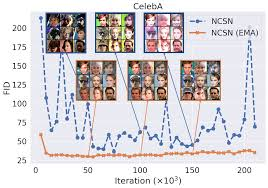
\includegraphics[width=0.7\textwidth]{figures/ema1.jpeg}
           \end{center} 
        \end{minipage}\begin{minipage}{0.5\textwidth}
        \begin{center}
            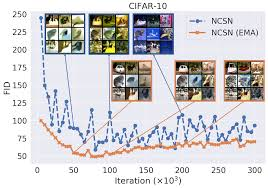
\includegraphics[width=0.7\textwidth]{figures/ema2.jpeg}
            \end{center}
        \end{minipage}
            Inestabilidades en el entrenamiento. Imagen extraída de \citet{SongErmon2020}.
        \end{center}
    \end{frame}
    
%----------------------------------------------------------------------------------------
% Final PAGE
% Set the text that is showed on the final slide
\finalpagetext{¡Gracias por su atención!}
%----------------------------------------------------------------------------------------
\makefinalpage

\begin{frame}{}
\begin{center}
    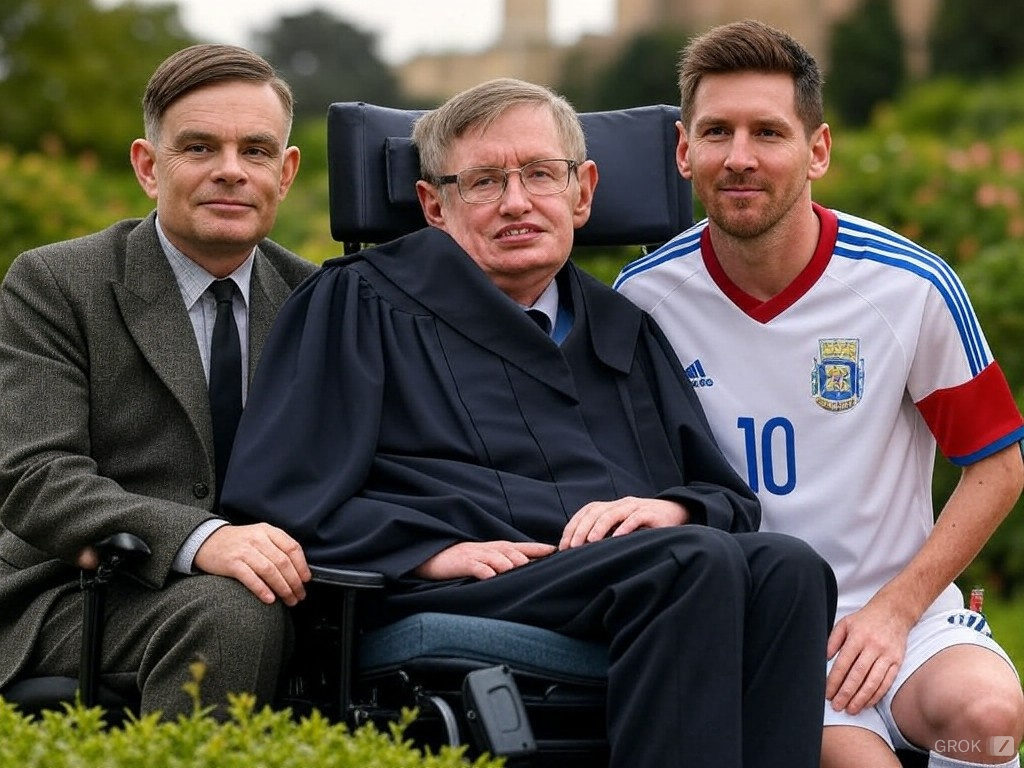
\includegraphics[width=0.7\textwidth]{figures/TuringHawkingMessi.jpeg}
\end{center}
    
\end{frame}

\begin{frame}[allowframebreaks, noframenumbering]{Referencias}
    \footnotesize{
        \begin{thebibliography}{99}

            \bibitem[Anderson, 1982]{Anderson1982} Anderson, B. D. O. (1982).
            \newblock Reverse-time diffusion equation models.
            \newblock \emph{Stochastic Processes and their Applications}, 12(3):313–326.
            
            \bibitem[Arjovsky et al., 2017]{Arjovsky2017} Arjovsky, M., Chintala, S., \& Bottou, L. (2017).
            \newblock Wasserstein generative adversarial networks.
            \newblock \emph{Proceedings of the 34th International Conference on Machine Learning}, PMLR, 70, 214-223.

            \bibitem[Bakry et al., 2014]{Bakry2014} Bakry, D., Gentil, I., Ledoux, M., et al. (2014).
            \newblock Analysis and geometry of Markov diffusion operators.
            \newblock \emph{Springer}, volume 103.

            \bibitem[Balaji et al., 2022]{Balaji2022} Balaji, Y., et al. (2022).
            \newblock ediffi: Text-to-image diffusion models with an ensemble of expert denoisers.
            \newblock \emph{arXiv preprint arXiv:2211.01324}.

            \bibitem[Brock et al., 2019]{Brock2019} Brock, A., Donahue, J., \& Simonyan, K. (2019).
            \newblock Large Scale GAN Training for High Fidelity Natural Image Synthesis.
            \newblock \emph{International Conference on Learning Representations (ICLR) 2019}.

            \bibitem[Cattiaux et al., 2021]{Cattiaux2021} Cattiaux, P., Conforti, G., Gentil, I., \& Léonard, C. (2021).
            \newblock Time reversal of diffusion processes under a finite entropy condition.
            \newblock \emph{arXiv preprint arXiv:2104.07708}.

            \bibitem[Chen et al., 2022]{Chen2022} Chen, S., Chewi, S., Li, J., Li, Y., Salim, A., \& Zhang, A. R. (2022).
            \newblock Sampling is as easy as learning the score: theory for diffusion models with minimal data assumptions.
            \newblock \emph{arXiv preprint arXiv:2209.11215}.

            \bibitem[Chen et al., 2023]{Chen2023} Chen, M., Huang, K., Zhao, T., \& Wang, M. (2023).
            \newblock Score approximation, estimation and distribution recovery of diffusion models on low-dimensional data.
            \newblock \emph{arXiv preprint arXiv:2302.07194}.

            \bibitem[Dalalyan, 2017]{Dalalyan2017} Dalalyan, A. S. (2017).
            \newblock Theoretical guarantees for approximate sampling from smooth and log-concave densities.
            \newblock \emph{Journal of the Royal Statistical Society: Series B (Statistical Methodology)}, 79(3):651–676.

            \bibitem[De Bortoli, 2022]{DeBortoli2022} De Bortoli, V. (2022).
            \newblock Convergence of denoising diffusion models under the manifold hypothesis.
            \newblock \emph{arXiv preprint arXiv:2208.05314}.

            \bibitem[De Bortoli et al., 2021a]{DeBortoli2021a} De Bortoli, V., Doucet, A., Heng, J., \& Thornton, J. (2021a).
            \newblock Simulating diffusion bridges with score matching.
            \newblock \emph{arXiv preprint arXiv:2111.07243}.

            \bibitem[De Bortoli et al., 2021b]{DeBortoli2021b} De Bortoli, V., Thornton, J., Heng, J., \& Doucet, A. (2021b).
            \newblock Diffusion schrödinger bridge with applications to score-based generative modeling.
            \newblock \emph{Advances in Neural Information Processing Systems}, 34.

            \bibitem[Dhariwal \& Nichol, 2021]{DhariwalNichol2021} Dhariwal, P., \& Nichol, A. (2021).
            \newblock Diffusion models beat gans on image synthesis.
            \newblock \emph{Advances in Neural Information Processing Systems}, 34.

            \bibitem[Durham \& Gallant, 2002]{DurhamGallant2002} Durham, G. B., \& Gallant, A. R. (2022).
            \newblock Numerical techniques for maximum likelihood estimation of continuous-time diffusion processes.
            \newblock \emph{Journal of Business \& Economic Statistics}, 20(3):297–338.

            \bibitem[Durmus \& Moulines, 2017]{DurmusMoulines2017} Durmus, A., \& Moulines, É. (2017).
            \newblock Nonasymptotic convergence analysis for the unadjusted Langevin algorithm.
            \newblock \emph{Annals of Applied Probability}, 27(3):1551–1587.

            \bibitem[Efron, 2011]{Efron2011} Efron, B. (2011).
            \newblock Tweedie's formula and selection bias.
            \newblock \emph{Journal of the American Statistical Association}, 106(496):1602–1614.
            
            \bibitem[Gao et al., 2020]{Gao2020} Gao, R., Song, Y., Poole, B., Wu, Y. N., \& Kingma, D. P. (2020).
            \newblock Learning energy-based models by diffusion recovery likelihood.
            \newblock \emph{arXiv preprint arXiv:2012.08125}.
            
            \bibitem[Goodfellow et al., 2014]{Goodfellow2014} Goodfellow, I., et al. (2014).
            \newblock Generative Adversarial Networks.
            \newblock \emph{Advances in Neural Information Processing Systems 27 (NIPS 2014)}.

            \bibitem[Google, 2024a]{GoogleGAN} Google. (2024a).
            \newblock Overview of GAN Structure.
            \newblock \emph{Machine Learning - Google for Developers}. Accedido 10-05-2024. Dirección: \url{https://developers.google.com/machine-learning/gan/gan_structure}

            \bibitem[Gulrajani et al., 2017]{Gulrajani2017} Gulrajani, I., Ahmed, F., Arjovsky, M., Dumoulin, V., \& Courville, A. (2017).
            \newblock Improved Training of Wasserstein GANs.
            \newblock \emph{Advances in Neural Information Processing Systems 30 (NIPS 2017)}.

            \bibitem[Haussmann \& Pardoux, 1986]{HaussmannPardoux1986} Haussmann, U. G., \& Pardoux, E. (1986).
            \newblock Time reversal of diffusions.
            \newblock \emph{The Annals of Probability}, pages 1188–1205.
            
            \bibitem[Heusel et al., 2017]{Heusel2017} Heusel, M., Ramsauer, H., Unterthiner, T., Nessler, B., \& Hochreiter, S. (2017).
            \newblock GANs Trained by a Two Time-Scale Update Rule Converge to a Local Nash Equilibrium.
            \newblock \emph{Neural Information Processing Systems (NIPS)}.

            \bibitem[Ho \& Salimans, 2021]{HoSalimans2021} Ho, J., \& Salimans, T. (2021).
            \newblock Classifier-free diffusion guidance.
            \newblock \emph{NeurIPS 2021 Workshop on Deep Generative Models and Downstream Applications}.

            \bibitem[Ho et al., 2020]{Ho2020} Ho, J., Jain, A., \& Abbeel, P. (2020).
            \newblock Denoising diffusion probabilistic models.
            \newblock \emph{Advances in Neural Information Processing Systems}, 33:6840–6851.

            \bibitem[Huang et al., 2021]{Huang2021} Huang, C.-W., Lim, J. H., \& Courville, A. C. (2021).
            \newblock A variational perspective on diffusion-based generative models and score matching.
            \newblock \emph{Advances in Neural Information Processing Systems}, 34.

            \bibitem[Hyvärinen, 2005]{Hyvarinen2005} Hyvärinen, A. (2005).
            \newblock Estimation of non-normalized statistical models by score matching.
            \newblock \emph{Journal of Machine Learning Research}, 6(4).

            \bibitem[Ikeda \& Watanabe, 2014]{IkedaWatanabe2014} Ikeda, N., \& Watanabe, S. (2014).
            \newblock Stochastic differential equations and diffusion processes.
            \newblock \emph{Elsevier}.
            
            \bibitem[Isola et al., 2016]{Isola2016} Isola, P., Zhu, J.-Y., Zhou, T., \& Efros, A. A. (2016).
            \newblock Image-to-Image Translation with Conditional Adversarial Networks.
            \newblock \emph{IEEE Conference on Computer Vision and Pattern Recognition (CVPR) 2017}.

            \bibitem[Karras et al., 2017]{Karras2017} Karras, T., Aila, T., Laine, S., \& Lehtinen, J. (2017).
            \newblock Progressive Growing of GANs for Improved Quality, Stability, and Variation.
            \newblock \emph{International Conference on Learning Representations (ICLR) 2018}.

            \bibitem[Karras et al., 2019]{Karras2019} Karras, T., Laine, S., \& Aila, T. (2019).
            \newblock A Style-Based Generator Architecture for Generative Adversarial Networks.
            \newblock \emph{IEEE Conference on Computer Vision and Pattern Recognition (CVPR) 2019}.

            \bibitem[Karras et al., 2022]{Karras2022} Karras, T., Aittala, M., Aila, T., \& Laine, S. (2022).
            \newblock Elucidating the design space of diffusion-based generative models.
            \newblock \emph{arXiv preprint arXiv:2206.00364}.

            \bibitem[Lee et al., 2022]{Lee2022} Lee, H., Lu, J., \& Tan, Y. (2022).
            \newblock Convergence for score-based generative modeling with polynomial complexity.
            \newblock \emph{arXiv preprint arXiv:2206.06227}.

            \bibitem[Luhman \& Luhman, 2021]{Luhman2021} Luhman, E. \& Luhman, T. (2021).
            \newblock Knowledge distillation in iterative generative models for improved sampling speed.
            \newblock \emph{arXiv preprint arXiv:2101.02388}.
            
            \bibitem[Meng et al., 2022]{Meng2022} Meng, C., Gao, R., Kingma, D. P., Ermon, S., Ho, J. \& Salimans, T. (2022).
            \newblock On distillation of guided diffusion models.
            \newblock \emph{arXiv preprint arXiv:2210.03142}.

            \bibitem[Muñoz López, 2024]{MunozLopez2024} Muñoz López, F. I. (2024).
            \newblock \emph{Cálculo del baricentro de Wasserstein bayesiano en conjuntos de imágenes mediante el descenso del gradiente estocástico}.
            \newblock Memoria para optar al título de Ingeniero Civil Matemático, Universidad de Chile.

            \bibitem[Nichol \& Dhariwal, 2021]{NicholDhariwal2021} Nichol, A. Q., \& Dhariwal, P. (2021).
            \newblock Improved denoising diffusion probabilistic models.
            \newblock \emph{International Conference on Machine Learning}, pages 8162–8171. PMLR.

            \bibitem[Pidstrigach, 2022]{Pidstrigach2022} Pidstrigach, J. (2022).
            \newblock Score-based generative models detect manifolds.
            \newblock \emph{arXiv preprint arXiv:2206.01018}.

            \bibitem[Poole et al., 2022]{Poole2022} Poole, B., Jain, A., Barron, J. T., \& Mildenhall, B. (2022).
            \newblock Dreamfusion: Text-to-3d using 2d diffusion.
            \newblock \emph{arXiv preprint arXiv:2209.14988}.

            \bibitem[Radford et al., 2015]{Radford2015} Radford, A., Metz, L., \& Chintala, S. (2015).
            \newblock Unsupervised Representation Learning with Deep Convolutional Generative Adversarial Networks.
            \newblock \emph{International Conference on Learning Representations (ICLR) 2016}.

            \bibitem[Radford et al., 2021]{Radford2021} Radford, A., et al. (2021).
            \newblock Learning transferable visual models from natural language supervision.
            \newblock \emph{International conference on machine learning}, pages 8748–8763. PMLR.

            \bibitem[Ramesh et al., 2022]{Ramesh2022} Ramesh, A., Dhariwal, P., Nichol, A., Chu, C., \& Chen, M. (2022).
            \newblock Hierarchical text-conditional image generation with clip latents.
            \newblock \emph{arXiv preprint arXiv:2204.06125}.

            \bibitem[Rombach et al., 2022]{Rombach2022} Rombach, R., Blattmann, A., Lorenz, D., Esser, P., \& Ommer, B. (2022).
            \newblock High-resolution image synthesis with latent diffusion models.
            \newblock \emph{Proceedings of the IEEE/CVF Conference on Computer Vision and Pattern Recognition}, pages 10684–10695.
            
            \bibitem[Saharia et al., 2022]{Saharia2022} Saharia, C., et al. (2022).
            \newblock Photorealistic text-to-image diffusion models with deep language understanding.
            \newblock \emph{arXiv preprint arXiv:2205.11487}.

            \bibitem[Salimans et al., 2016]{Salimans2016} Salimans, T., et al. (2016).
            \newblock Improved Techniques for Training GANs.
            \newblock \emph{Advances in Neural Information Processing Systems 29 (NIPS 2016)}.
            
            \bibitem[Salimans \& Ho, 2022]{SalimansHo2022} Salimans, T. \& Ho, J. (2022).
            \newblock Progressive distillation for fast sampling of diffusion models.
            \newblock \emph{arXiv preprint arXiv:2202.00512}.
            
            \bibitem[San Martín-Arastegui, 2018]{SanMartin2018} San Martín-Arastegui, J. (2018).
            \newblock \emph{Teoría de la Medida}, 1.ª ed.
            \newblock Editorial Universitaria. ISBN: 978-956-11-2577-3.

            \bibitem[Santana, 2017]{Santana2017} Santana, C. (2017).
            \newblock Creando Caras Artificiales Con Gans mejoradas: Data Coffee \#4.
            \newblock Accedido 10-01-2024. Dirección: \url{https://youtu.be/bMDpMRB7CEs?si=JtMHA9kZ3uKrK14T&t=272}

            \bibitem[Sohl-Dickstein et al., 2015]{Sohl-Dickstein2015} Sohl-Dickstein, J., Weiss, E., Maheswaranathan, N., \& Ganguli, S. (2015).
            \newblock Deep unsupervised learning using nonequilibrium thermodynamics.
            \newblock \emph{International Conference on Machine Learning}, pages 2256–2265. PMLR.

            \bibitem[Song \& Ermon, 2019]{SongErmon2019} Song, Y., \& Ermon, S. (2019).
            \newblock Generative modeling by estimating gradients of the data distribution.
            \newblock \emph{Advances in Neural Information Processing Systems}, 32.

            \bibitem[Song \& Ermon, 2020]{SongErmon2020} Song, Y., \& Ermon, S. (2020).
            \newblock Improved techniques for training score-based generative models.
            \newblock \emph{Advances in neural information processing systems}, 33:12438–12448.

            \bibitem[Song et al., 2020a]{Song2020a} Song, J., Meng, C., \& Ermon, S. (2020a).
            \newblock Denoising diffusion implicit models.
            \newblock \emph{arXiv preprint arXiv:2010.02502}.

            \bibitem[Song et al., 2020b]{Song2020b} Song, Y., Sohl-Dickstein, J., Kingma, D. P., Kumar, A., Ermon, S., \& Poole, B. (2020b).
            \newblock Score-based generative modeling through stochastic differential equations.
            \newblock \emph{arXiv preprint arXiv:2011.13456}.

            \bibitem[Song et al., 2021]{Song2021} Song, Y., Durkan, C., Murray, I., \& Ermon, S. (2021).
            \newblock Maximum likelihood training of score-based diffusion models.
            \newblock \emph{Advances in Neural Information Processing Systems}, 34.
            
            \bibitem[Stroock \& Varadhan, 1997]{StroockVaradhan1997} Stroock, D. W. \& Varadhan, S. R. S. (1997).
            \newblock Multidimensional diffusion processes.
            \newblock \emph{Springer Science \& Business Media}, volume 233.

            \bibitem[Vincent, 2011]{Vincent2011} Vincent, P. (2011).
            \newblock A connection between score matching and denoising autoencoders.
            \newblock \emph{Neural Computation}, 23(7):1661–1674.

            \bibitem[Wang et al., 2018]{Wang2018} Wang, X., Yu, K., Wu, S., Gu, J., Liu, Y., Dong, C., Qiao, Y., \& Loy, C. C. (2018).
            \newblock ESRGAN: Enhanced Super-Resolution Generative Adversarial Networks.
            \newblock \emph{European Conference on Computer Vision (ECCV)}.

            \bibitem[Watson et al., 2021]{Watson2021} Watson, D., Ho, J., Norouzi, M., \& Chan, W. (2021).
            \newblock Learning to efficiently sample from diffusion probabilistic models.
            \newblock \emph{arXiv preprint arXiv:2106.03802}.

            \bibitem[Wikipedia, 2024b]{WikipediaGAN} Wikipedia. (2024b).
            \newblock Generative adversarial network - Wikipedia.
            \newblock Accedido 09-05-2024. Dirección: \url{https://en.wikipedia.org/wiki/Generative_adversarial_network}

            \bibitem[Xiao et al., 2021]{Xiao2021} Xiao, Z., Kreis, K., \& Vahdat, A. (2021).
            \newblock Tackling the generative learning trilemma with denoising diffusion gans.
            \newblock \emph{arXiv preprint arXiv:2112.07804}.
            
            \bibitem[Zhu et al., 2017]{Zhu2017} Zhu, J.-Y., Park, T., Isola, P., \& Efros, A. A. (2017).
            \newblock Unpaired Image-to-Image Translation using Cycle-Consistent Adversarial Networks.
            \newblock \emph{International Conference on Computer Vision (ICCV) 2017}.

        \end{thebibliography}
    }
\end{frame}

%----------------------------------------------------------------------------------------
\end{document}